\documentclass{scalatekids-article}
\usepackage[italian]{babel}
\usepackage{tocloft}
\cftsetindents{paragraph}{4em}{5em}
\cftsetindents{subparagraph}{5em}{6em}
\begin{document}
\lfoot{Specifica Tecnica 1.0.0}
\newgeometry{top=3.5cm}
\begin{titlepage}
  \begin{center}
    \begin{center}
      
\includegraphics[width=10cm]{sklogo.png}
    \end{center}
    \vspace{1cm}
    \begin{Huge}
      \begin{center}
        \textbf{Specifica Tecnica}
      \end{center}
    \end{Huge}
    \vspace{11pt}
    \bgroup
    \def\arraystretch{1.3}
    \begin{tabular}{r|l}
      \multicolumn{2}{c}{\textbf{Informazioni sul documento}} \\
      \hline
      \setbox0=\hbox{0.0.1\unskip}\ifdim\wd0=0pt
      \\
      \else
      \textbf{Versione} & 1.0.0\\
      \fi
      \textbf{Redazione} & \multiLineCell[t]{}\\
      \textbf{Verifica} & \multiLineCell[t]{}\\
      \textbf{Approvazione} & \multiLineCell[t]{}\\
      \textbf{Uso} & Esterno\\
      \textbf{Lista di Distribuzione} & \multiLineCell[t]{ScalateKids\\Prof. Tullio Vardanega\\Prof. Riccardo Cardin}\\
    \end{tabular}
    \egroup
    \vspace{22pt}
  \end{center}
\end{titlepage}
\restoregeometry
\clearpage
\pagenumbering{Roman}
\setcounter{page}{1}
\begin{flushleft}
  \vspace{0cm}
  {\large\bfseries Diario delle modifiche \par}
\end{flushleft}
\vspace{0cm}
\begin{center}
  \begin{tabular}{| l | l | l | l | p{5cm} |}
    \hline
    Versione & Autore & Ruolo & Data & Descrizione \\
    \hline
    0.4.0 & Michael Munaro & Verificatore & 2016-03-25 & Verifica sezione 5\\
    \hline
    0.3.1 & Giacomo Vanin & Progettista & 2016-03-24 & Stesura sezione 5\\
    \hline
    0.3.0 & Alberto De Agostini & Verificatore & 2016-03-22 & Verifica sezioni da 4.6 a 4.13\\
    \hline
    0.2.2 & Marco Boseggia & Progettista & 2016-03-22 & Stesura sezioni 4.10 4.11 4.12 4.13\\
    \hline
    0.2.1 & Marco Boseggia & Progettista & 2016-03-21 & Stesura sezioni 4.6 4.7 4.8 4.9\\
    \hline
    0.2.0 & Michael Munaro & Verificatore & 2016-03-21 & Verifica sottosezioni 3.1 3.2 4.1 4.2 4.3 4.4 4.5\\
    \hline
    0.1.2 & Andrea Giacomo Baldan & Progettista & 2016-03-17 & Stesura sottosezioni 4.1 4.2 4.3 4.4 4.5\\
    \hline
    0.1.1 & Andrea Giacomo Baldan & Progettista & 2016-03-17 & Stesura sottosezioni 3.1 3.2\\
    \hline
    0.1.0 & Michael Munaro & Verificatore & 2016-03-16 & Verifica sezioni 1 e 2\\
    \hline
    0.0.2 & Marco Boseggia & Progettista & 2016-02-26 & Stesura sezioni 1 e 2\\
    \hline
    0.0.1 & Andrea Giacomo Baldan & Amministratore & 2016-02-26 & Creazione scheletro del documento\\
    \hline
  \end{tabular}
\end{center}
\newpage
\tableofcontents
\newpage
\pagenumbering{arabic}

\section{Sommario}

\subsection{Scopo del documento}

Il seguente documento ha lo scopo di descrivere la progettazione ad alto livello
che il gruppo \textit{ScalateKids} ha scelto per il
progetto \textbf{ActorBase}.\\  Sarà descritta l'\gloss{architettura} generale
del progetto, in particolare  la scelta dei \gloss{design pattern} e delle
componentiche andranno a comporre il software.

\prodPurpose

\glossExpl

\subsection{Riferimenti}

\subsubsection{Normativi}

\begin{itemize}

\item\textbf{Capitolato d'appalto C1:} \textit{Actorbase: a NoSQL DB based on the Actor model;}\\
  \url{http://www.math.unipd.it/~tullio/IS-1/2015/Progetto/C1.pdf}
\item\textbf{Norme di Progetto:}
  \href{run:../Interni/NormeDiProgetto\_v2.0.0.pdf}{Norme di Progetto v2.0.0.}
\end{itemize}

\subsubsection{Informativi}

\begin{itemize}
\item\textbf{Piano di Progetto:}
  \href{run:./PianoDiProgetto\_v2.0.0.pdf}{Piano di Progetto v2.0.0}
\item\textbf{Dispense fornite dall'insegnamento Ingegneria del Software mod.
    A:}\\   \url{http://www.math.unipd.it/~tullio/IS-1/2015/}
\item\textbf{Documentazione di \gloss{Akka} su \gloss{Scala}:}
  \url{http://doc.akka.io/docs/akka/2.4.2/scala.html}
\item\textbf{Scala Pickling - Fast, Customizable, Boilerplate-Free Serialization for Scala:}
  \url{http://lampwww.epfl.ch/~hmiller/pickling}
\item\textbf{RESP - Redis Protocol Specification:}
  \url{http://redis.io/topics/protocol}
\end{itemize}

\newpage

\section{Tecnologie utilizzate}

In questa sezione saranno descritte le tecnologie scelte per lo sviluppo del
progetto \textbf{ActorBase} e le motivazioni che ci hanno spinto a sceglierle.

\subsection{Akka}

La scelta della libreria \gloss{Akka} è stata dettata dal capitolato, tuttavia
l'avremmo scelta comunque per i seguenti motivi:
\begin{itemize}
\item\textbf{Implementazione del \gloss{modello ad attori}:} \gloss{Akka}
  rende semplice la creazione e l'utilizzo degli \gloss{attori}. Grazie a ciò è
  possibile creare facilmente architetture ad eventi estremamente concorrenti e
  viene naturale la distribuibilità del progetto e l'asincronia tra i processi;
\item\textbf{Tolleranza agli errori:} \gloss{Akka} implementa un sistema di
  gerarchia di supervisori. Questa gerarchia consente ai supervisori di un
  \gloss{attore}, nel caso in cui quest'ultimo lanci un'eccezione, di mandarlo
  in \gloss{crash} e farlo poi ripartire. In questo modo il sistema è resiliente
  agli errori;
\item\textbf{Persistenza:} Ogni messaggio ricevuto da ciascun \gloss{attore}
  può essere salvato in maniera tale che al riavvio esso possa riprendere dallo
  stato precedente al suo spegnimento.
\end{itemize}

\subsection{Scala}

Il capitolato richiede l'utilizzo di un linguaggio di programmazione a scelta
tra \gloss{Scala} e \gloss{Java}. Abbiamo scelto \gloss{Scala} per i seguenti
motivi:

\begin{itemize}
\item\textbf{\gloss{Programmazione funzionale}:} Questa tecnica di
  programmazione evita che ci siano degli effetti collaterali tra funzioni,
  rendendole quindi \gloss{thread-safe};
\item\textbf{Implementazione di Akka:} \gloss{Akka} risulta più
  facilmente implementabile in \gloss{Scala} che in \gloss{Java}. Questo perchè
  la \gloss{programmazione funzionale} con i suoi paradigmi si integra meglio
  con il \gloss{modello ad attori};
\item\textbf{Implementazione di DSL:} Scala si presta alla creazione di \gloss{DSL}
  in maniera nativa, sia di tipo esterno che di tipo interno, senza necessariamente
  utilizzare librerie esterne o appoggiarsi a framework appositi.
\end{itemize}

\section{Descrizione architettura}

\subsection{Metodo e formalismo di specifica}

L'esposizione dell'architettura segue la metodologia \gloss{top-down},
descrivendo l'architettura iniziando dalle componenti generali e scendendo
nel dettaglio. Seguirà quindi la descrizione dei \gloss{package} seguiti dalla descrizione
in dettaglio delle classi e interfacce che vi appartengono, specificando
per ognuna la funzione e le relazioni in ingresso ed uscita. Il formalismo
cromatico utilizzato sarà conforme a quanto specificato in \textit{Norme Di Progetto}.\\
Successivamente si illustreranno i \gloss{Design Pattern} e la loro applicazione
all'interno delle componenti, con un approfondimento del loro funzionamento
in \hyperref[sec:appendice]{appendice A}.\\
Nel trattare le componenti, si chiarisce che sono da intendersi come \gloss{package}
e i due termini verranno quindi usati come sinonimi.\\

\subsection{Architettura generale}

Macroscopicamente il sistema si suddivide in due componenti principali,
assimilabili ad un paradigma Client-Server, il sistema ad attori dove risiedono
la struttura della base di dati ed un server TCP (Transmission Control Protocol)
pronto a ricevere comandi dall'esterno rappresentano la componente server, la
Command Line Interface (CLI) rappresenta la componente client mediante la quale
è possibile inviare comandi al sistema e ricevere l'output prodotto da essi,
essa farà uso della componente \gloss{driver} per comunicare con il sistema lato
server mediante il protocollo di comunicazione testuale \hyperref[sec:RESP]{RESP}.\\

\begin{figure}[H]
  \begin{center}
    \includegraphics[width=0.2\textwidth,keepaspectratio]{RP/RP-ClientServer.png}
    \caption{Diagramma architettura concettuale}
  \end{center}
\end{figure}

Questo ha portato alla suddivisione del progetto in tre macro-componenti, rispettivamente
\textbf{cli}, \textbf{driver} e \textbf{actorsystem}; contenute all'interno del package
generale \textbf{actorbase}.

\begin{figure}[H]
  \begin{center}
    \includegraphics[width=0.9\textwidth,keepaspectratio]{RP/Architettura-AltoLivello.png}
    \caption{Diagramma componenti principali}
  \end{center}
\end{figure}

\subsection{Protocollo di comunicazione Client-Server}
\label{sec:RESP}

\textbf{Actorbase} è stato concepito come sistema da utilizzare in ambiente
affidabile, e non dovrebbe essere esposto direttamente alla rete internet, ma
utilizzato all'interno di sottoreti protette dall'esterno, per questo è stato
deciso di riutilizzare un protocollo di comunicazione
piuttosto semplice, leggero e facilmente comprensibile.\\
Il protocollo \gloss{\textbf{RESP}} (REdis Serialization Protocol) implementato
dal \gloss{database} \gloss{REDIS} si presta esattamente allo scopo, utilizza
5 tipi di dato differenziati dal primo \gloss{byte} che li compone, e delimitati
da una sequenza di terminazione formata da \gloss{CR} (Carriage Return) e \gloss{LF}
(Line Feed) che rappresenta il carattere ``a capo'':
\begin{itemize}
\item \textbf{Simple Strings} rappresentano stringhe dedicate alle risposte
  semplici (\gloss{ack} dei comandi ricevuti), non possono contenere caratteri
  di terminazione al loro interno; il primo byte è ``+'';
\item \textbf{Errors} rappresentano stringhe di errore, formate da:
  \begin{center}
    \verb=-TIPOERRORE MESSAGGIOERRORE\r\n=
  \end{center}
  verranno utilizzate per generare le eccezioni lato client; il primo byte è ``-'';
\item \textbf{Integers} rappresentano numeri interi, il primo byte è ``:'';
\item \textbf{Bulk Strings} rappresentano stringhe dedicate al \gloss{payload}, formate da:
  \begin{center}
    \verb=\$LUNGHEZZAPAYLOAD\r\nPAYLOAD\r\n=
  \end{center}
  il primo byte è ``\$'' e può contenere caratteri di ``a capo'';
\item \textbf{Arrays} rappresentano \gloss{array} di comandi e \textbf{Bulk String}, formati da:
  \begin{center}
    \verb=*LUNGHEZZASTRINGA\r\nRESPSTRING\r\n=
  \end{center}
 il primo byte è ``*'', possono contenere qualsiasi altro tipo di stringa \gloss{RESP}, inclusi altri \gloss{array}.
\end{itemize}

\section{Componenti}

\subsection{actorbase}
\label{sec:actorbase}

\subsubsection{Descrizione}

La componente principale rappresentata dal package globale \textbf{actorbase}.

\subsubsection{Package contenuti}

\begin{itemize}
\item \hyperref[sec:actorbase::cli]{actorbase::cli};
\item \hyperref[sec:actorbase::driver]{actorbase::driver};
\item \hyperref[sec:actorbase::actorsystem]{actorbase::actorsystem}.
\end{itemize}

Rappresentano le tre macro-componenti del sistema.

%%%%%%%%%%%%%%%%%%%%%%%%%%%%%%%%%%%%%%%%%%%%%%%%%%%%%%%%%%%%%%%%%%%%
%                      ACTORSYSTEM PARTE                           %
%%%%%%%%%%%%%%%%%%%%%%%%%%%%%%%%%%%%%%%%%%%%%%%%%%%%%%%%%%%%%%%%%%%%

\subsection{actorbase::actorsystem}
\label{sec:actorbase::actorsystem}

\subsubsection{Descrizione}

\gloss{Package} che raggruppa tutte le componenti del sistema che
rappresentano il \gloss{server}.

\subsubsection{Package contenuti}

\begin{itemize}
\item \hyperref[sec:actorbase::actorsystem::clientactor]{actorbase::actorsystem::clientactor};
\item \hyperref[sec:actorbase::actorsystem::tcpserver]{actorbase::actorsystem::tcpserver};
\item \hyperref[sec:actorbase::actorsystem::storefinder]{actorbase::actorsystem::storefinder};
\item \hyperref[sec:actorbase::actorsystem::storekeeper]{actorbase::actorsystem::storekeeper};
\item \hyperref[sec:actorbase::actorsystem::warehouseman]{actorbase::actorsystem::warehouseman};
\item \hyperref[sec:actorbase::actorsystem::ninja]{actorbase::actorsystem::ninja};
\item \hyperref[sec:actorbase::actorsystem::manager]{actorbase::actorsystem::manager};
\item \hyperref[sec:actorbase::actorsystem::userkeeper]{actorbase::actorsystem::userkeeper};
\item \hyperref[sec:actorbase::actorsystem::main]{actorbase::actorsystem::main};
\item \hyperref[sec:actorbase::actorsystem::serialization]{actorbase::actorsystem::serialization}.
\end{itemize}

\subsubsection{Interazioni con altre componenti}

\begin{itemize}
\item \hyperref[sec:actorbase::driver]{actorbase::driver};
\item Akka.
\end{itemize}

\subsection{actorbase::actorsystem::clientactor}
\label{sec:actorbase::actorsystem::clientactor}

\subsubsection{Descrizione}

\gloss{Package} per l'attore con cui si interfaccerà il \gloss{driver}.

\subsubsection{Package contenuti}

\begin{itemize}
\item \hyperref[sec:actorbase::actorsystem::clientactor::messages]{actorbase::actorsystem::clientactor::messages}.
\end{itemize}

\subsubsection{Classi}

\paragraph{actorbase::actorsystem::clientactor::ClientActor}
\label{sec:actorbase::actorsystem::clientactor::ClientActor}

\subparagraph{Descrizione}

Classe che rappresenta l'attore con cui si interfaccia il \gloss{driver} dopo
la connessione.

\subparagraph{Utilizzo}

Questo attore riceve le richieste da \hyperref[sec:actorbase::driver::client::Connection]{actorbase::driver::client::Connection}
e si occupa di inviare messaggi a \hyperref[sec:actorbase::actorsystem::main::Main]{actorbase::actorsystem::main::Main}.

\subparagraph{Classi ereditate}

\begin{itemize}

\item akka::actor::Actor.

\end{itemize}

\subparagraph{Interazioni con altre classi}

\begin{itemize}
\item \hyperref[sec:actorbase::actorsystem::serialization::SerializationContext]{actorbase::actorsystem::serialization::SerializationContext};
\item \hyperref[sec:actorbase::actorsystem::serialization::DeserializationContext]{actorbase::actorsystem::serialization::DeserializationContext};
\item akka::actor::ActorRef.
\end{itemize}

\subsection{actorbase::actorsystem::clientactor::messages}
\label{sec:actorbase::actorsystem::clientactor::messages}

\subsubsection{Descrizione}

\gloss{Package} che contiene tutti i messaggi che possono essere ricevuti da
\hyperref[sec:actorbase::actorsystem::clientactor::ClientActor]{actorbase::actorsystem::clientactor::ClientActor}.

\subsubsection{Classi}

\paragraph{actorbase::actorsystem::clientactor::messages::LoginResponse}
\label{sec:actorbase::actorsystem::clientactor::messages::LoginResponse}

\subparagraph{Descrizione}

Messaggio che contiene la password di un utente che ha richiesto il login.

\subparagraph{Utilizzo}

In seguito alla ricezione di questo messaggio l'attore di tipo
\hyperref[sec:actorbase::actorsystem::clientactor::ClientActor]{actorbase::actorsystem::clientactor::ClientActor}
controlla che la password ricevuta sia uguale a quella immessa
dall'utente e, in caso affermativo, cambia il proprio stato.

\paragraph{actorbase::actorsystem::clientactor::messages::PeerClosed}
\label{sec:actorbase::actorsystem::clientactor::messages::PeerClosed}

\subparagraph{Descrizione}

Messaggio che indica la volontà di chiudere la connessione con il \gloss{driver}.

\subparagraph{Utilizzo}

In seguito alla ricezione di questo messaggio l'attore di tipo
\hyperref[sec:actorbase::actorsystem::actorclient::ActorClient]{actorbase::actorsystem::actorclient::ActorClient}
chiude la connessione con il \gloss{driver} e termina.

\paragraph{actorbase::actorsystem::clientactor::messages::RESPInput}
\label{sec:actorbase::actorsystem::clientactor::messages::RESPInput}

\subparagraph{Descrizione}

Messaggio che rappresenta l'input ricevuto dal \gloss{driver}.

\subparagraph{Utilizzo}

In seguito alla ricezione di questo messaggio l'attore di tipo
\hyperref[sec:actorbase::actorsystem::clientactor::ClientActor]{actorbase::actorsystem::clientactor::ClientActor}
deserializza il messaggio sfruttando la componente
\hyperref[sec:actorbase::actorsystem::serialization::DeserializationContext]{actorbase::actorsystem::serialization::DeserializationContext}.
Dopo aver fatto ciò crea il messaggio corrispondente al tipo di richiesta che gli era arrivato
e lo manda all'attore \hyperref[sec:actorbase::actorsystem::main::Main]{actorbase::actorsystem::main::Main}.

\paragraph{actorbase::actorsystem::clientactor::messages::UpdateReadCollections}
\label{sec:actorbase::actorsystem::clientactor::messages::UpdateReadCollections}

\subparagraph{Descrizione}

Messaggio che indica la necessità di aggiornare l'insieme delle
\gloss{collezioni} cui l'utente ha permessi di sola lettura.

\subparagraph{Utilizzo}

Quando \hyperref[sec:actorbase::actorsystem::clientactor::ClientActor]{actorbase::actorsystem::clientactor::ClientActor}
riceve questo messaggio aggiorna la sua lista di \gloss{collezioni}
cui l'utente ha permessi di sola lettura aggiungendo la
\gloss{collezione} presente nel messaggio.

\paragraph{actorbase::actorsystem::clientactor::messages::UpdateCollections}
\label{sec:actorbase::actorsystem::clientactor::messages::UpdateCollections}

\subparagraph{Descrizione}

Messaggio che indica la necessità di aggiornare l'insieme delle
\gloss{collezioni} cui l'utente ha permessi di lettura e scrittura.

\subparagraph{Utilizzo}

Quando \hyperref[sec:actorbase::actorsystem::clientactor::ClientActor]{actorbase::actorsystem::clientactor::ClientActor}
riceve questo messaggio aggiorna la sua lista di \gloss{collezioni}
cui l'utente ha permessi di lettura e scrittura aggiungendo
la \gloss{collezione} presente nel messaggio.

\paragraph{actorbase::actorsystem::clientactor::messages::Response}
\label{sec:actorbase::actorsystem::clientactor::messages::Response}

\subparagraph{Descrizione}

Messaggio che rappresenta la risposta da parte del \gloss{server} da inoltrare
al \gloss{driver}.

\subparagraph{Utilizzo}

Quando \hyperref[sec:actorbase::actorsystem::clientactor::ClientActor]{actorbase::actorsystem::clientactor::ClientActor}
riceve questo messaggio il contenuto di quest'ultimo viene serializzato tramite
\hyperref[sec:actorbase::actorsystem::serialization::DeserializationContext]{actorbase::actorsystem::serialization::DeserializationContext}
e mandato a \hyperref[sec:actorbase::driver::client::Connection]{actorbase::driver::\allowbreak{}client::\allowbreak{}Connection}.

\subsection{actorbase::actorsystem::tcpactor}
\label{sec:actorbase::actorsystem::tcpactor}

\subsubsection{Descrizione}

\gloss{Package} per l'attore con cui si interfaccerà il \gloss{driver} per la connessione iniziale.

\subsubsection{Package contenuti}

\begin{itemize}
\item \hyperref[sec:actorbase::actorsystem::tcpserver::messages]{actorbase::actorsystem::tcpserver::messages}.
\end{itemize}

\subsubsection{Classi}

\paragraph{actorbase::actorsystem::tcpserver::TCPServer}
\label{sec:actorbase::actorsystem::tcpserver::TCPServer}

\subparagraph{Descrizione}

Classe che rappresenta l'attore con cui si interfaccia il \gloss{driver} per
istanziare la connessione.

\subparagraph{Utilizzo}

Questo attore riceve la richiesta di connessione da
\hyperref[sec:actorbase::driver::client::Connection]{actorbase::driver::client::Connection}
e si occupa di associare al \gloss{client} un attore di tipo
\hyperref[sec:actorbase::actorsystem::clientactor::ClientActor]{actorbase::actorsystem::clientactor::ClientActor}
per continuare le comunicazioni.

\subparagraph{Classi ereditate}

\begin{itemize}

\item akka::actor::Actor.

\end{itemize}

\subsection{actorbase::actorsystem::tcpserver::messages}
\label{sec:actorbase::actorsystem::tcpserver::messages}

\subsubsection{Descrizione}

\gloss{Package} che contiene tutti i messaggi che possono essere ricevuti da
\hyperref[sec:actorbase::actorsystem::tcpserver::TCPServer]{actorbase::actorsystem::tcpserver::TCPServer}.

\subsubsection{Classi}

\paragraph{actorbase::actorsystem::tcpserver::messages::Bound}
\label{sec:actorbase::actorsystem::tcpserver::messages::Bound}

\subparagraph{Descrizione}

Messaggio che rappresenta la necessità di mettere il \gloss{server} in ascolto.

\subparagraph{Utilizzo}

Quando \hyperref[sec:actorbase::actorsystem::tcpserver::TCPServer]{actorbase::actorsystem::tcpserver::TCPServer}
riceve questo messaggio si mette in ascolto su una porta del \gloss{server}.

\paragraph{actorbase::actorsystem::tcpserver::messages::CommandFailed}
\label{sec:actorbase::actorsystem::tcpserver::messages::CommandFailed}

\subparagraph{Descrizione}

Messaggio che rappresenta un errore nella comunicazione \gloss{TCP}.

\subparagraph{Utilizzo}

Quando \hyperref[sec:actorbase::actorsystem::tcpserver::TCPServer]{actorbase::actorsystem::tcpserver::TCPServer}
riceve questo messaggio manderà una notifica a
\hyperref[sec:actorbase::driver::client::Connection]{actorbase::driver::client::Connection}.

\paragraph{actorbase::actorsystem::tcpserver::messages::Connected}
\label{sec:actorbase::actorsystem::tcpserver::messages::Connected}

\subparagraph{Descrizione}

Messaggio che rappresenta una connessione \gloss{TCP} riuscita.

\subparagraph{Utilizzo}

Quando \hyperref[sec:actorbase::actorsystem::tcpserver::TCPServer]{actorbase::actorsystem::tcpserver::TCPServer}
riceve questo messaggio associa al \gloss{client} un attore di tipo
\hyperref[sec:actorbase::actorsystem::clientactor::ClientActor]{actorbase::actorsystem::clientactor::ClientActor}.

\subsection{actorbase::actorsystem::serialization}
\label{sec:actorbase::actorsystem::serialization}

\subsubsection{Descrizione}

\gloss{Package} che si occupa di \gloss{serializzare} e \gloss{deserializzare}
i messaggi mandati o ricevuti dal \gloss{driver}.

\subsubsection{Interazioni con altre componenti}

\begin{itemize}

\item \hyperref[sec:actorbase::actorsystem::warehouseman]{actorbase::actorsystem::warehouseman};
\item \hyperref[sec:actorbase::actorsystem::clientactor]{actorbase::actorsystem::clientactor}.

\end{itemize}

\subsubsection{Classi}

\paragraph{actorbase::actorsystem::serialization::SerializationContext}
\label{sec:actorbase::actorsystem::serialization::SerializationContext}

\subparagraph{Descrizione}

Classe che offre dei metodi per la scelta su quale tipo di \gloss{serializzazione}
effettuare.

\subparagraph{Utilizzo}

Questa classe viene utilizzata da \hyperref[sec:actorbase::actorsystem::warehouseman::Warehouseman]{actorbase::\allowbreak{}actorsystem::\allowbreak{}warehouseman::\allowbreak{}Warehouseman}
e \hyperref[sec:actorbase::actorsystem::clientactor::ClientActor]{actorbase::\allowbreak{}actorsystem::\allowbreak{}clientactor::\allowbreak{}ClientActor}
per \gloss{serializzare} i dati scegliendo una tra le strategie indicate
dalle classi che estendono \hyperref[sec:actorbase::actorsystem::serialization::SerializationStrategy]{actorbase::\allowbreak{}actorsystem::\allowbreak{}serialization::\allowbreak{}SerializationStrategy}.

\subparagraph{Interazioni con altre classi}

\begin{itemize}

\item \hyperref[sec:actorbase::actorsystem::warehouseman::Warehouseman]{actorbase::actorsystem::warehouseman::Warehouseman};
\item \hyperref[sec:actorbase::actorsystem::clientactor::ClientActor]{actorbase::actorsystem::clientactor::ClientActor};
\item \hyperref[sec:actorbase::actorsystem::serialization::SerializationStrategy]{actorbase::actorsystem::serialization::SerializationStrategy}.

\end{itemize}

\paragraph{actorbase::actorsystem::serialization::SerializationStrategy}
\label{sec:actorbase::actorsystem::serialization::SerializationStrategy}

\subparagraph{Descrizione}

Interfaccia che offre una strategia generale per \gloss{serializzare} i dati.

\subparagraph{Utilizzo}

Questa interfaccia viene utilizzata per l'applicazione del \gloss{designpattern}
\gloss{strategy}. Offre un metodo generalizzato per la
\gloss{serializzazione} di dati che verrà poi implementato dalle classi che
implementeranno questa interfaccia.

\subparagraph{Interazioni con altre classi}

\begin{itemize}

\item \hyperref[sec:actorbase::actorsystem::serialization::SerializationContext]{actorbase::actorsystem::serialization::SerializationContext}.

\end{itemize}

\paragraph{actorbase::actorsystem::serialization::RESPSerialization}
\label{sec:actorbase::actorsystem::serialization::RESPSerialization}

\subparagraph{Descrizione}

Classe che si occupa di serializzare i dati in stringhe di formato \gloss{RESP}.

\subparagraph{Utilizzo}

Questa classe viene utilizzata per l'implementazione di una strategia di
serializzazione in formato \gloss{RESP}. Viene utilizzata principalmente per
dati che dovranno essere mandati al \gloss{driver}.

\subparagraph{Classi ereditate}

\begin{itemize}

\item \hyperref[sec:actorbase::actorsystem::serialization::SerializationStrategy]{actorbase::actorsystem::serialization::SerializationStrategy}.

\end{itemize}

\paragraph{actorbase::actorsystem::serialization::PickleSerialization}
\label{sec:actorbase::actorsystem::serialization::PickleSerialization}

\subparagraph{Descrizione}

Classe che si occupa di serializzare i dati in formato \gloss{Pickle}.

\subparagraph{Utilizzo}

Questa classe viene utilizzata per l'implementazione di una strategia di
serializzazione in formato \gloss{Pickle}. Viene utilizzata principalmente per
dati che dovranno essere salvati su disco.

\subparagraph{Classi ereditate}

\begin{itemize}

\item \hyperref[sec:actorbase::actorsystem::serialization::SerializationStrategy]{actorbase::actorsystem::serialization::SerializationStrategy}.

\end{itemize}

\paragraph{actorbase::actorsystem::serialization::DeserializationContext}
\label{sec:actorbase::actorsystem::serialization::DeserializationContext}

\subparagraph{Descrizione}

Classe che offre dei metodi per la scelta su quale tipo di \gloss{deserializzazione}
effettuare.

\subparagraph{Utilizzo}

Questa classe viene utilizzata da \hyperref[sec:actorbase::actorsystem::warehouseman::Warehouseman]{actorbase::actorsystem::warehouseman::Warehouseman}
e \hyperref[sec:actorbase::actorsystem::clientactor::ClientActor]{actorbase::\allowbreak{}actorsystem::\allowbreak{}clientactor::\allowbreak{}ClientActor}
per \gloss{deserializzare} i dati scegliendo una tra le strategie indicate
dalle classi che estendono \hyperref[sec:actorbase::actorsystem::serialization::DeserializationStrategy]{actorbase::\allowbreak{}actorsystem::\allowbreak{}serialization::\allowbreak{}DeserializationStrategy}.

\subparagraph{Interazioni con altre classi}

\begin{itemize}

\item \hyperref[sec:actorbase::actorsystem::warehouseman::Warehouseman]{actorbase::actorsystem::warehouseman::Warehouseman};
\item \hyperref[sec:actorbase::actorsystem::clientactor::ClientActor]{actorbase::actorsystem::clientactor::ClientActor};
\item \hyperref[sec:actorbase::actorsystem::serialization::DeserializationStrategy]{actorbase::actorsystem::serialization::DeserializationStrategy}.

\end{itemize}

\paragraph{actorbase::actorsystem::serialization::DeserializationStrategy}
\label{sec:actorbase::actorsystem::serialization::DeserializationStrategy}

\subparagraph{Descrizione}

Interfaccia che offre una strategia generale per \gloss{deserializzare} i dati.

\subparagraph{Utilizzo}

Questa interfaccia viene utilizzata per l'applicazione del \gloss{design pattern}
\gloss{strategy}. Offre un metodo generalizzato per la
\gloss{deserializzazione} di dati che verrà poi implementato dalle classi che
implementeranno questa interfaccia.

\subparagraph{Interazioni con altre classi}

\begin{itemize}

\item \hyperref[sec:actorbase::actorsystem::serialization::DeserializationContext]{actorbase::actorsystem::serialization::DeserializationContext}.

\end{itemize}

\paragraph{actorbase::actorsystem::serialization::RESPDeserialization}
\label{sec:actorbase::actorsystem::serialization::RESPDeserialization}

\subparagraph{Descrizione}

Classe che si occupa di deserializzare i dati da stringhe in formato \gloss{RESP}.

\subparagraph{Utilizzo}

Questa classe viene utilizzata per l'implementazione di una strategia di
\gloss{deserializzazione} dal formato \gloss{RESP}. Viene utilizzato
principalmente per i dati ricevuti dal \gloss{driver}.

\subparagraph{Classi ereditate}

\begin{itemize}

\item \hyperref[sec:actorbase::actorsystem::serialization::DeserializationStrategy]{actorbase::actorsystem::serialization::DeserializationStrategy}.

\end{itemize}

\paragraph{actorbase::actorsystem::serialization::PickleDeserialization}
\label{sec:actorbase::actorsystem::serialization::PickleDeserialization}

\subparagraph{Descrizione}

Classe che si occupa di \gloss{deserializzare} i dati dal formato \gloss{Pickle}.

\subparagraph{Utilizzo}

Questa classe viene utilizzata per l'implementazione di una strategia di
\gloss{deserializzazione} dal formato \gloss{Pickle}. Viene utilizzato
principalmente per la lettura di dati da disco.

\subparagraph{Classi ereditate}

\begin{itemize}

\item \hyperref[sec:actorbase::actorsystem::serialization::DeserializationStrategy]{actorbase::actorsystem::serialization::DeserializationStrategy}.

\end{itemize}

\subsection{actorbase::actorsystem::warehouseman}
\label{sec:actorbase::actorsystem::warehouseman}

\subsubsection{Descrizione}

\gloss{Package} che rappresenta l'attore che si occuperà della
\gloss{persistenza} su disco dei dati.

\subsubsection{Package contenuti}

\begin{itemize}

\item \hyperref[sec:actorbase::actorsystem::warehouseman::messages]{actorbase::actorsystem::warehouseman::messages}.

\end{itemize}

\subsubsection{Classi}

\paragraph{actorbase::actorsystem::warehouseman::Warehouseman}
\label{sec:actorbase::actorsystem::warehouseman::Warehouseman}

\subparagraph{Descrizione}

Classe che rappresenta un \gloss{attore} di tipo \gloss{Warehouseman}.

\subparagraph{Utilizzo}

Questa classe viene utilizzata per effettuare il salvataggio su filesystem del
\gloss{database} e per caricare i dati da filesystem.

\subparagraph{Classi ereditate}

\begin{itemize}

\item akka::actor::Actor.

\end{itemize}

\subparagraph{Interazioni con altre classi}

\begin{itemize}
\item \hyperref[sec:actorbase::actorsystem::serialization::SerializationContext]{actorbase::actorsystem::serialization::SerializationContext};
\item \hyperref[sec:actorbase::actorsystem::serialization::DeserializationContext]{actorbase::actorsystem::serialization::DeserializationContext};
\item akka::actor::ActorRef.
\end{itemize}

\subsection{actorbase::actorsystem::warehouseman::messages}
\label{sec:actorbase::actorsystem::warehouseman::messages}

\subsubsection{Descrizione}

\gloss{Package} che racchiude tutti i messaggi che gli attori di tipo
\gloss{Warehouseman} possono ricevere.

\paragraph{actorbase::actorsystem::warehouseman::messages::Init}
\label{sec:actorbase::actorsystem::warehouseman::messages::Init}

\subparagraph{Descrizione}

Messaggio che porta alla lettura dei dati da disco.

\subparagraph{Utilizzo}

Quando \hyperref[sec:actorbase::actorsystem::warehouseman::Warehouseman]{actorbase::actorsystem::warehouseman::Warehouseman}
riceve questo messaggio inizializza uno \hyperref[sec:actorbase::actorsystem::storekeeper::StoreKeeper]{actorbase::actorsystem::storekeeper::StoreKeeper}
con i dati letti da disco.

\paragraph{actorbase::actorsystem::warehouseman::messages::Save}
\label{sec:actorbase::actorsystem::warehouseman::messages::Save}

\subparagraph{Descrizione}

Messaggio che porta al salvataggio dei dati su disco.

\subparagraph{Utilizzo}

Quando \hyperref[sec:actorbase::actorsystem::warehouseman::Warehouseman]{actorbase::actorsystem::warehouseman::Warehouseman}
riceve questo messaggio salverà i dati su disco sfruttando
\hyperref[sec:actorbase::actorsystem::serialization::SerializationContext]{actorbase::actorsystem::serialization::SerializationContext}.

\subsection{actorbase::actorsystem::main}
\label{sec:actorbase::actorsystem::main}

\subsubsection{Descrizione}

\gloss{Package} che rappresenta l'attore che si occuperà di gestire le
richieste al \gloss{server}.

\subsubsection{Package contenuti}

\begin{itemize}

\item \hyperref[sec:actorbase::actorsystem::main::messages]{actorbase::actorsystem::main::messages}.

\end{itemize}

\subsubsection{Classi}

\paragraph{actorbase::actorsystem::main::Main}
\label{sec:actorbase::actorsystem::main::Main}

\subparagraph{Descrizione}

Classe che rappresenta un \gloss{attore} di tipo \gloss{Main}.

\subparagraph{Utilizzo}

Questa classe viene utilizzata per gestire le richieste ricevute al
\gloss{server}.

\subparagraph{Classi ereditate}

\begin{itemize}

\item akka::actor::Actor.

\end{itemize}

\subparagraph{Interazioni con altre classi}

\begin{itemize}
\item akka::actor::ActorRef.
\end{itemize}

\subsection{actorbase::actorsystem::main::messages}
\label{sec:actorbase::actorsystem::main::messages}

\subsubsection{Descrizione}

\gloss{Package} che racchiude tutti i messaggi che gli attori di tipo
\gloss{Warehouseman} possono ricevere.

\subsubsection{Package importati}

\begin{itemize}
\item \hyperref[sec:actorbase::actorsystem::storefinder::messages]{actorbase::actorsystem::storefinder::messages}
\end{itemize}

\paragraph{actorbase::actorsystem::main::messages::CreateCollection}
\label{sec:actorbase::actorsystem::main::messages::CreateCollection}

\subparagraph{Descrizione}

Messaggio che porta alla creazione di una \gloss{collezione}.

\subparagraph{Utilizzo}

Quando \hyperref[sec:actorbase::actorsystem::main::Main]{actorbase::actorsystem::main::Main}
riceve questo messaggio inizializza uno \hyperref[sec:actorbase::actorsystem::storefinder::Storefinder]{actorbase::actorsystem::\allowbreak{}storefinder::\allowbreak{}Storefinder}.

\paragraph{actorbase::actorsystem::main::messages::GetCollection}
\label{sec:actorbase::actorsystem::main::messages::GetCollection}

\subparagraph{Descrizione}

Messaggio che indica una richiesta di una \gloss{collezione}.

\subparagraph{Utilizzo}

Quando \hyperref[sec:actorbase::actorsystem::main::Main]{actorbase::actorsystem::main::Main}
riceve questo messaggio cercherà l'attore di tipo
\hyperref[sec:actorbase::actorsystem::storefinder::Storefinder]{actorbase::actorsystem::\allowbreak{}storefinder::\allowbreak{}Storefinder}
corrispondente alla \gloss{collezione} cercata.

\paragraph{actorbase::actorsystem::main::messages::RemoveCollection}
\label{sec:actorbase::actorsystem::main::messages::RemoveCollection}

\subparagraph{Descrizione}

Messaggio che indica una richiesta di rimozione di una \gloss{collezione}.

\subparagraph{Utilizzo}

Quando \hyperref[sec:actorbase::actorsystem::main::Main]{actorbase::actorsystem::main::Main}
riceve questo messaggio cercherà l'attore di tipo
\hyperref[sec:actorbase::actorsystem::storefinder::Storefinder]{actorbase::actorsystem::\allowbreak{}storefinder::\allowbreak{}Storefinder}
corrispondente alla \gloss{collezione} cercata e ne avvierà
la procedura di rimozione dal \gloss{database}.

\paragraph{actorbase::actorsystem::main::messages::GetItemFrom}
\label{sec:actorbase::actorsystem::main::messages::GetItemFrom}

\subparagraph{Descrizione}

Messaggio che indica una richiesta di ricerca di un \gloss{item} da una o più \gloss{collezione}.

\subparagraph{Utilizzo}

Quando \hyperref[sec:actorbase::actorsystem::main::Main]{actorbase::actorsystem::main::Main}
riceve questo messaggio cercherà gli attori di tipo
\hyperref[sec:actorbase::actorsystem::storefinder::Storefinder]{actorbase::actorsystem::\allowbreak{}storefinder::\allowbreak{}Storefinder}
corrispondenti alle \gloss{collezioni} su cui effettuare la ricerca
e inoltrerà a loro la richiesta dell'\gloss{item} con la chiave da cercare.

\paragraph{actorbase::actorsystem::main::messages::AddContributor}
\label{sec:actorbase::actorsystem::main::messages::AddContributor}

\subparagraph{Descrizione}

Messaggio che indica una richiesta di aggiunta di un collaboratore ad una
\gloss{collezione}.

\subparagraph{Utilizzo}

Quando \hyperref[sec:actorbase::actorsystem::main::Main]{actorbase::actorsystem::main::Main}
riceve questo messaggio cercherà gli attori di tipo
\hyperref[sec:actorbase::actorsystem::storefinder::Storefinder]{actorbase::actorsystem::\allowbreak{}storefinder::\allowbreak{}Storefinder}
che mappano gli attori di tipo \hyperref[sec:actorbase::actorsystem::storefinder::Storefinder]{actorbase::actorsystem::\allowbreak{}userkeeper::\allowbreak{}Userkeeper}.
e inoltrerà loro la richiesta di aggiunta del collaboratore.

\paragraph{actorbase::actorsystem::main::messages::DuplicateRequestSF}
\label{sec:actorbase::actorsystem::main::messages::DuplicateRequestSF}

\subparagraph{Descrizione}

Messaggio che indica una richiesta di sdoppiamento di uno \gloss{Storefinder}.

\subparagraph{Utilizzo}

Quando \hyperref[sec:actorbase::actorsystem::main::Main]{actorbase::actorsystem::main::Main}
riceve questo messaggio provvederà a sdoppiare l'attore di tipo
\hyperref[sec:actorbase::actorsystem::storefinder::Storefinder]{actorbase::actorsystem::\allowbreak{}storefinder::\allowbreak{}Storefinder}.

\paragraph{actorbase::actorsystem::main::messages::RemoveContributor}
\label{sec:actorbase::actorsystem::main::messages::RemoveContributor}

\subparagraph{Descrizione}

Messaggio che indica una richiesta di rimozione di un collaboratore ad una
\gloss{collezione}.

\subparagraph{Utilizzo}

Quando \hyperref[sec:actorbase::actorsystem::main::Main]{actorbase::actorsystem::main::Main}
riceve questo messaggio cercherà gli attori di tipo
\hyperref[sec:actorbase::actorsystem::storefinder::Storefinder]{actorbase::actorsystem::\allowbreak{}storefinder::\allowbreak{}Storefinder}
che mappano gli attori di tipo \hyperref[sec:actorbase::actorsystem::storefinder::Storefinder]{actorbase::actorsystem::\allowbreak{}userkeeper::\allowbreak{}Userkeeper}
e inoltrerà loro la richiesta di rimozione del collaboratore.

\paragraph{actorbase::actorsystem::main::messages::InitUserkeeper}
\label{sec:actorbase::actorsystem::main::messages::InitUserkeeper}

\subparagraph{Descrizione}

Messaggio che indica una richiesta di creazione di uno \gloss{Userkeeper}.

\subparagraph{Utilizzo}

Quando \hyperref[sec:actorbase::actorsystem::main::Main]{actorbase::actorsystem::main::Main}
riceve questo messaggio provvederà a inoltrare agli attori di tipo
\hyperref[sec:actorbase::actorsystem::storefinder::Storefinder]{actorbase::actorsystem::\allowbreak{}storefinder::\allowbreak{}Storefinder}
che mappano gli attori di tipo \hyperref[sec:actorbase::actorsystem::storefinder::Storefinder]{actorbase::actorsystem::\allowbreak{}userkeeper::\allowbreak{}Userkeeper}
la creazione di un attore di questo tipo.

%%%%%%%%%%%%%%%%%%%%%%%%%%%%%%%%%%%%%%%%%%%%%%%%%%%%%%%%%%%%%%%%%
%                  DA QUI A DRIVER DA CANCELLARE                %
%%%%%%%%%%%%%%%%%%%%%%%%%%%%%%%%%%%%%%%%%%%%%%%%%%%%%%%%%%%%%%%%%


\paragraph{actorbase::model::system::actors::Storefinder}

\subparagraph{Descrizione}

Classe che rappresenta un \gloss{attore} di tipo \gloss{Storefinder}.

\subparagraph{Utilizzo}

Viene utilizzata per tenere traccia dei contenuti degli attori di tipo
\gloss{Storekeeper}.

\subparagraph{Classi ereditate}

\begin{itemize}
\item actorbase::model::system::actors::Actor.
\end{itemize}

\paragraph{actorbase::model::system::actors::MainActor}

\subparagraph{Descrizione}

Classe che rappresenta un \gloss{attore} di tipo \gloss{MainActor}.

\subparagraph{Utilizzo}

Viene utilizzata per tenere traccia dei contenuti degli attori di tipo
\gloss{Storefinder}.

\subparagraph{Classi ereditate}

\begin{itemize}
\item actorbase::model::system::actors::Storefinder.
\end{itemize}

\paragraph{actorbase::model::system::actors::Storekeeper}

\subparagraph{Descrizione}

Classe che rappresenta un \gloss{attore} di tipo \gloss{Storekeeper}.

\subparagraph{Utilizzo}

Viene utilizzata per contenere gli elementi all'interno del \gloss{database}.

\subparagraph{Classi ereditate}

\begin{itemize}
\item actorbase::model::system::actors::Actor.
\end{itemize}

\paragraph{actorbase::model::system::actors::Manager}

\subparagraph{Descrizione}

Classe che rappresenta un \gloss{attore} di tipo \gloss{Manager}.

\subparagraph{Utilizzo}

Viene utilizzata per effettuare procedure di \gloss{load balancing}.

\subparagraph{Classi ereditate}

\begin{itemize}
\item actorbase::model::system::actors::Actor.
\end{itemize}

\paragraph{actorbase::model::system::actors::Ninja}

\subparagraph{Descrizione}

Classe che rappresenta un \gloss{attore} di tipo \gloss{Ninja}.

\subparagraph{Utilizzo}

Viene utilizzata per consentire di effettuare un \gloss{backup} dei contenuti
degli attori di tipo \gloss{Storekeeper}.

\subparagraph{Classi ereditate}

\begin{itemize}
\item actorbase::model::system::actors::Actor.
\end{itemize}

%%%%%%%%%%%%%%%%%%%%%%%%%%%%%%%%%%%%%%%%%%%%%%%%%%%%%%%%%%%%%%%%%%%%
%                        DRIVER PARTE                              %
%%%%%%%%%%%%%%%%%%%%%%%%%%%%%%%%%%%%%%%%%%%%%%%%%%%%%%%%%%%%%%%%%%%%

\subsection{actorbase::driver}
\label{sec:actorbase::driver}

\subsubsection{Descrizione}

\gloss{Package} per la componente \gloss{driver} dell'architettura
\gloss{MVC}.

\subsubsection{Interazioni con altre componenti}

\begin{itemize}
\item \hyperref[sec:actorbase::cli]{actorbase::cli};
\item \hyperref[sec:actorbase::actorsystem]{actorbase::actorsystem}.
\end{itemize}

\subsubsection{Package contenuti}

\begin{itemize}
\item \hyperref[sec:actorbase::driver::client]{actorbase::driver::client};
\item \hyperref[sec:actorbase::driver::serializer]{actorbase::driver::serializer};
\item \hyperref[sec:actorbase::driver::actorbasedata]{actorbase::driver::actorbasedata};
\item \hyperref[sec:actorbase::driver::exceptions]{actorbase::driver::exceptions}.
\end{itemize}

\subsection{actorbase::driver::client}
\label{sec:actorbase::driver::client}

\subsubsection{Descrizione}

\gloss{Package} che si occupa di comunicare sia con la componente \gloss{cli}
che con la componente \gloss{server} del sistema.

\subsubsection{Interazioni con altre componenti}

\begin{itemize}
\item \hyperref[sec:actorbase::cli::models]{actorbase::cli::models};
\item \hyperref[sec:actorbase::actorsystem::clientactor]{actorbase::actorsystem::clientactor}.
\end{itemize}

\subsubsection{Classi}

\paragraph{actorbase::driver::client::ActorbaseClient}
\label{sec:actorbase::driver::client::ActorbaseClient}

\subparagraph{Descrizione}

Classe che rappresenta un'istanza del \gloss{driver}.

\subparagraph{Utilizzo}

La componente \hyperref[sec:actorbase::cli::models::CommandReceiver]{actorbase::cli::models::CommandReceiver}
ha un riferimento a questa classe tramite il quale le vengono passati
i comandi che sono stati già sottoposti al \gloss{parsing}. Questa
classe si occupa di mandare il comando alla componente
\hyperref[sec:actorbase::driver::client::CommandRunner]{actorbase::driver::client::CommandRunner},
che rappresenta una classe \gloss{façade}, per farne proseguire l'esecuzione.\\
Il risultato delle operazioni viene restituito a \hyperref[sec:actorbase::cli::models::CommandReceiver]{actorbase::cli::models::CommandReceiver}
tramite oggetti di tipo \hyperref[sec:actorbase::driver::actorbasedata::ActorbaseObject]{actorbase::driver::actorbasedata::ActorbaseObject}.

\subparagraph{Interazioni con altre classi}

\begin{itemize}
\item \hyperref[sec:actorbase::cli::models::CommandReceiver]{actorbase::cli::models::CommandReceiver};
\item \hyperref[sec:actorbase::driver::client::CommandRunner]{actorbase::driver::client::CommandRunner};
\item \hyperref[sec:actorbase::driver::actorbasedata::ActorbaseObject]{actorbase::driver::actorbasedata::ActorbaseObject}.
\end{itemize}

\paragraph{actorbase::driver::client::CommandRunner}
\label{sec:actorbase::driver::client::CommandRunner}

\subparagraph{Descrizione}

Classe \gloss{façade} che si occupa di mettere in comunicazione il
\gloss{driver} con il \gloss{server}.

\subparagraph{Utilizzo}

Questa classe riceve dalla componente \hyperref[sec:actorbase::driver::client::ActorbaseClient]{actorbase::driver::client::ActorbaseClient}
il comando da eseguire e le restituisce il risultato nascondendole
tutte le operazioni eseguite.

\subparagraph{Interazioni con altre classi}

\begin{itemize}
\item \hyperref[sec:actorbase::driver::client::ActorbaseClient]{actorbase::driver::client::ActorbaseClient};
\item \hyperref[sec:actorbase::driver::client::Connection]{actorbase::driver::client::Connection}.
\end{itemize}

\paragraph{actorbase::driver::client::Connection}
\label{sec:actorbase::driver::client::Connection}

\subparagraph{Descrizione}

Classe per la connessione tra il \gloss{driver} e il \gloss{server}.

\subparagraph{Utilizzo}

Questa classe si incarica della connessione e comunicazione con il \gloss{server}. Una volta
connesso alla componente \hyperref[sec:actorbase::actorsystem::tcpserver::TCPServer]{actorbase::actorsystem::\allowbreak{}tcpserver::\allowbreak{}TCPServer}
le verrà assegnato un oggetto di tipo \hyperref[sec:actorbase::actorsystem::clientactor::ClientActor]{actorbase::\allowbreak{}actorsystem::\allowbreak{}clientactor::\allowbreak{}ClientActor}.\\
Questa classe inoltre chiamerà le componenti necessarie per la serializzazione e deserializzazione
delle stringhe ricevute dal \gloss{server} o da \hyperref[sec:actorbase::driver::client::CommandRunner]{actorbase::\allowbreak{}driver::\allowbreak{}client::\allowbreak{}CommandRunner},
ossia \hyperref[sec:actorbase::driver::serializer::SerializationContext]{actorbase::\allowbreak{}driver::\allowbreak{}serializer::\allowbreak{}SerializationContext}
e \hyperref[sec:actorbase::driver::serializer::Deserializationtext]{actorbase::\allowbreak{}driver::\allowbreak{}serializer::\allowbreak{}DeserializationContext}.

\subparagraph{Interazioni con altre classi}
\begin{itemize}
\item \hyperref[sec:actorbase::driver::serializer::SerializationContext]{actorbase::driver::serializer::SerializationContext};
\item \hyperref[sec:actorbase::driver::serializer::Deserializationtext]{actorbase::driver::serializer::DeserializationContext};
\item \hyperref[sec:actorbase::driver::client::CommandRunner]{actorbase::driver::client::CommandRunner};
\item \hyperref[sec:actorbase::actorsystem::tcpserver::TCPServer]{actorbase::actorsystem::tcpserver::TCPServer};
\item \hyperref[sec:actorbase::actorbase::actorsystem::clientactor::ClientActor]{actorbase::actorsystem::clientactor::ClientActor}.
\end{itemize}

\subsection{actorbase::driver::serializer}
\label{sec:actorbase::driver::serializer}

\subsubsection{Descrizione}

\gloss{Package} che si occupa di \gloss{serializzare} e \gloss{deserializzare}
i messaggi mandati o ricevuti dal \gloss{server}.

\subsubsection{Interazioni con altre componenti}

\begin{itemize}

\item \hyperref[sec:actorbase::driver::client]{actorbase::driver::client};
\item \hyperref[sec:actorbase::driver::actorbasedata]{actorbase::driver::actorbasedata}.

\end{itemize}

\subsubsection{Classi}

\paragraph{actorbase::driver::serializer::SerializationContext}
\label{sec:actorbase::driver::serializer::SerializationContext}

\subparagraph{Descrizione}

Classe che offre dei metodi per la scelta su quale tipo di \gloss{serializzazione}
effettuare.

\subparagraph{Utilizzo}

Questa classe viene utilizzata da \hyperref[sec:actorbase::driver::client::Connection]{actorbase::driver::client::Connection}
per \gloss{serializzare} i dati scegliendo una tra le strategie indicate
dalle classi che estendono \hyperref[sec:actorbase::driver::serializer::SerializationStrategy]{actorbase::driver::serializer::SerializationStrategy}.

\subparagraph{Interazioni con altre classi}

\begin{itemize}

\item \hyperref[sec:actorbase::driver::client::Connection]{actorbase::driver::client::Connection};
\item \hyperref[sec:actorbase::driver::serializer::SerializationStrategy]{actorbase::driver::serializer::SerializationStrategy}.

\end{itemize}

\paragraph{actorbase::driver::serializer::SerializationStrategy}
\label{sec:actorbase::driver::serializer::SerializationStrategy}

\subparagraph{Descrizione}

Interfaccia che offre una strategia generale per \gloss{serializzare} i dati.

\subparagraph{Utilizzo}

Questa interfaccia viene utilizzata per l'applicazione del \gloss{design pattern}
\gloss{strategy}. Offre un metodo generalizzato per la
\gloss{serializzazione} di dati che verrà poi implementato dalle classi che
implementeranno questa interfaccia.

\subparagraph{Interazioni con altre classi}

\begin{itemize}

\item \hyperref[sec:actorbase::driver::serializer::SerializationContext]{actorbase::driver::serializer::SerializationContext}.

\end{itemize}

\paragraph{actorbase::driver::serializer::RESPSerialize}

\subparagraph{Descrizione}

Classe che si occupa di serializzare i dati in stringhe di formato \gloss{RESP}.

\subparagraph{Utilizzo}

Questa classe viene utilizzata per l'implementazione di una strategia di
serializzazione in formato \gloss{RESP}.

\subparagraph{Classi ereditate}

\begin{itemize}

\item \hyperref[sec:actorbase::driver::serializer::SerializationStrategy]{actorbase::driver::serializer::SerializationStrategy}.

\end{itemize}

\paragraph{actorbase::driver::serializer::DeserializationContext}
\label{sec:actorbase::driver::serializer::DeserializationContext}

\subparagraph{Descrizione}

Classe che offre dei metodi per la scelta su quale tipo di \gloss{deserializzazione}
effettuare.

\subparagraph{Utilizzo}

Questa classe viene utilizzata da \hyperref[sec:actorbase::driver::client::Connection]{actorbase::driver::client::Connection}
per \gloss{deserializzare} i dati scegliendo una tra le strategie indicate
dalle classi che estendono \hyperref[sec:actorbase::driver::serializer::DeserializationStrategy]{actorbase::driver::serializer::DeserializationStrategy}.

\subparagraph{Interazioni con altre classi}

\begin{itemize}

\item \hyperref[sec:actorbase::driver::serializer::DeserializationStrategy]{actorbase::driver::serializer::DeserializationStrategy}.

\end{itemize}

\paragraph{actorbase::driver::serializer::DeserializationStrategy}
\label{sec:actorbase::driver::serializer::DeserializationStrategy}

\subparagraph{Descrizione}

Interfaccia che offre una strategia generale per \gloss{deserializzare} i dati.

\subparagraph{Utilizzo}

Questa interfaccia viene utilizzata per l'applicazione del \gloss{design pattern}
\gloss{strategy}. Offre un metodo generalizzato per la
\gloss{deserializzazione} di dati che verrà poi implementato dalle classi che
implementeranno questa interfaccia.

\subparagraph{Interazioni con altre classi}

\begin{itemize}

\item \hyperref[sec:actorbase::driver::serializer::DeserializationContext]{actorbase::driver::serializer::DeserializationContext}.

\end{itemize}

\paragraph{actorbase::driver::serializer::RESPDeserialize}

\subparagraph{Descrizione}

Classe che si occupa di deserializzare i dati da stringhe in formato \gloss{RESP}.

\subparagraph{Utilizzo}

Questa classe viene utilizzata per l'implementazione di una strategia di
\gloss{deserializzazione} dal formato \gloss{RESP}.

\subparagraph{Classi ereditate}

\begin{itemize}

\item \hyperref[sec:actorbase::driver::serializer::DeserializationStrategy]{actorbase::driver::serializer::DeserializationStrategy}.

\end{itemize}

\subparagraph{Interazioni con altre classi}

\begin{itemize}

\item \hyperref[sec:actorbase::driver::actorbasedata::RESPArrayString]{actorbase::driver::actorbasedata::RESPArrayString}.

\end{itemize}

\subsection{actorbase::driver::actorbasedata}
\label{sec:actorbase::driver::actorbasedata}

\subsubsection{Descrizione}

\gloss{Package} che offre le strutture dati necessarie per la comunicazione
con il \gloss{server}, con la \gloss{cli} o eventuali programmi esterni.

\subsubsection{Interazioni con altre componenti}
\begin{itemize}
\item \hyperref[sec:actorbase::cli::models]{actorbase::cli::models};
\item \hyperref[sec:actorbase::driver::client]{actorbase::driver::client};
\item \hyperref[sec:actorbase::driver::serializer]{actorbase::driver::serializer}.
\end{itemize}

\subsubsection{Classi}

\paragraph{actorbase::driver::actorbasedata::ActorbaseObject}
\label{sec:actorbase::driver::actorbasedata::ActorbaseObject}

\subparagraph{Descrizione}

Interfaccia che rappresenta una struttura dati generica per ritornare i dati
ricevuti dal \gloss{server} alla \gloss{cli} o a un programma esterno.

\subparagraph{Utilizzo}

Questa interfaccia viene utilizzata dalle classi che la implementano per
rappresentare un insieme di \gloss{collezioni} o \gloss{item}.

\subparagraph{Interazioni con altre classi}

\begin{itemize}
\item \hyperref[sec:actorbase::driver::client::ActorbaseClient]{actorbase::driver::client::ActorbaseClient}.
\end{itemize}

\paragraph{actorbase::driver::actorbasedata::ActorbaseItem}
\label{sec:actorbase::driver::actorbasedata::ActorbaseItem}

\subparagraph{Descrizione}

Classe che implementa \hyperref[sec:actorbase::driver::actorbasedata::ActorbaseObject]{actorbase::driver::actorbasedata::ActorbaseObject}
in modo da rappresentare un singolo \gloss{item}.

\subparagraph{Utilizzo}

Questa classe viene utilizzata per la rappresentazione di un singolo
\gloss{item} che verrà restituito alla \gloss{cli} o a un programma esterno.

\subparagraph{Classi ereditate}

\begin{itemize}
\item \hyperref[sec:actorbase::driver::actorbasedata::ActorbaseObject]{actorbase::driver::actorbasedata::ActorbaseObject}.
\end{itemize}

\paragraph{actorbase::driver::actorbasedata::ActorbaseCollection}
\label{sec:actorbase::driver::actorbasedata::ActorbaseCollection}

\subparagraph{Descrizione}

Classe che implementa \hyperref[sec:actorbase::driver::actorbasedata::ActorbaseObject]{actorbase::driver::actorbasedata::ActorbaseObject}
in modo da rappresentare una singola \gloss{collezione}.

\subparagraph{Utilizzo}

Questa classe viene utilizzata per la rappresentazione di una singola
\gloss{collezione} vista come insieme di oggetti di tipo
\hyperref[sec:actorbase::driver::actorbasedata::ActorbaseItem]{actorbase::driver::actorbasedata::ActorbaseItem}
che verrà restituito alla \gloss{cli} o a un programma esterno.
Essa offrirà anche un \gloss{cursore} di tipo
\hyperref[sec:actorbase::driver::actorbasedata::ItemCursor]{actorbase::driver::actorbasedata::ItemCursor}
per scorrere gli \gloss{item} al suo interno.

\subparagraph{Classi ereditate}

\begin{itemize}
\item \hyperref[sec:actorbase::driver::actorbasedata::ActorbaseObject]{actorbase::driver::actorbasedata::ActorbaseObject}.
\end{itemize}

\subparagraph{Interazioni con altre classi}

\begin{itemize}
\item \hyperref[sec:actorbase::driver::actorbasedata::ActorbaseItem]{actorbase::driver::actorbasedata::ActorbaseItem};
\item \hyperref[sec:actorbase::driver::actorbasedata::ItemCursor]{actorbase::driver::actorbasedata::ItemCursor}.
\end{itemize}

\paragraph{actorbase::driver::actorbasedata::ActorbaseCollectionSeq}
\label{sec:actorbase::driver::actorbasedata::ActorbaseCollectionSeq}

\subparagraph{Descrizione}

Classe che implementa \hyperref[sec:actorbase::driver::actorbasedata::ActorbaseObject]{actorbase::driver::actorbasedata::ActorbaseObject}
in modo da rappresentare un insieme di \gloss{collezioni}.

\subparagraph{Utilizzo}

Questa classe viene utilizzata per la rappresentazione di un insieme di
\gloss{collezioni} viste come insieme di oggetti di tipo
\hyperref[sec:actorbase::driver::actorbasedata::ActorbaseCollection]{actorbase::driver::actorbasedata::ActorbaseCollection}
che verrà restituito alla \gloss{cli} o a un programma esterno.
Essa offrirà anche un \gloss{cursore} di tipo
\hyperref[sec:actorbase::driver::actorbasedata::CollectionCursor]{actorbase::driver::actorbasedata::CollectionCursor}
per scorrere le \gloss{collezioni} al suo interno.

\subparagraph{Classi ereditate}

\begin{itemize}
\item \hyperref[sec:actorbase::driver::actorbasedata::ActorbaseObject]{actorbase::driver::actorbasedata::ActorbaseObject}.
\end{itemize}

\subparagraph{Interazioni con altre classi}

\begin{itemize}
\item \hyperref[sec:actorbase::driver::actorbasedata::ActorbaseCollection]{actorbase::driver::actorbasedata::ActorbaseCollection};
\item \hyperref[sec:actorbase::driver::actorbasedata::CollectionCursor]{actorbase::driver::actorbasedata::CollectionCursor}.
\end{itemize}

\paragraph{actorbase::driver::actorbasedata::Cursor}
\label{sec:actorbase::driver::actorbasedata::Cursor}

\subparagraph{Descrizione}

Interfaccia che offre un cursore per lo scorrimento di una struttura dati
secondo il \gloss{design pattern} \gloss{iterator}.

\subparagraph{Utilizzo}

Questa interfaccia contiene i metodi necessari allo scorrimento di una
struttura dati.

\paragraph{actorbase::driver::actorbasedata::ItemCursor}
\label{sec:actorbase::driver::actorbasedata::ItemCursor}

\subparagraph{Descrizione}

Classe che offre al \gloss{driver} un cursore per lo scorrimento di una struttura dati
che rappresenta una singola \gloss{collezione} implementando l'interfaccia
\hyperref[sec:actorbase::driver::actorbasedata::Cursor]{actorbase::driver::actorbasedata::Cursor}.

\subparagraph{Utilizzo}

Questa classe viene utilizzata dalla classe
\hyperref[sec:actorbase::driver::actorbasedata::ActorbaseCollection]{actorbase::driver::actorbasedata::ActorbaseCollection}
per scorrere gli \gloss{item} interni alla \gloss{collezione}
rappresentata.

\subparagraph{Classi ereditate}

\begin{itemize}
\item \hyperref[sec:actorbase::driver::actorbasedata::Cursor]{actorbase::driver::actorbasedata::Cursor}.
\end{itemize}

\subparagraph{Interazioni con altre classi}

\begin{itemize}
\item \hyperref[sec:actorbase::driver::actorbasedata::ActorbaseCollection]{actorbase::driver::actorbasedata::ActorbaseCollection}.
\end{itemize}

\paragraph{actorbase::driver::actorbasedata::CollectionCursor}
\label{sec:actorbase::driver::actorbasedata::CollectionCursor}

\subparagraph{Descrizione}

Classe che offre al \gloss{driver} un cursore per lo scorrimento di una struttura dati
che rappresenta un'insieme di \gloss{collezioni} implementando l'interfaccia
\hyperref[sec:actorbase::driver::actorbasedata::Cursor]{actorbase::driver::actorbasedata::Cursor}.

\subparagraph{Utilizzo}

Questa classe viene utilizzata dalla classe
\hyperref[sec:actorbase::driver::actorbasedata::ActorbaseCollection]{actorbase::driver::actorbasedata::ActorbaseCollection}
per scorrere le \gloss{collezioni} interni all'insieme di \gloss{collezioni}
rappresentato.

\subparagraph{Classi ereditate}

\begin{itemize}
\item \hyperref[sec:actorbase::driver::actorbasedata::Cursor]{actorbase::driver::actorbasedata::Cursor}.
\end{itemize}

\subparagraph{Interazioni con altre classi}

\begin{itemize}
\item \hyperref[sec:actorbase::driver::actorbasedata::ActorbaseCollectionSeq]{actorbase::driver::actorbasedata::ActorbaseCollectionSeq}.
\end{itemize}

\paragraph{actorbase::driver::actorbasedata::RESPArrayString}
\label{sec:actorbase::driver::actorbasedata::RESPArrayString}

\subparagraph{Descrizione}

Questa classe rappresenta un \gloss{array} di
\hyperref[sec:actorbase::driver::actorbasedata::RESPSimpleString]{actorbase::driver::actorbasedata::RESPSimpleString}.

\subparagraph{Utilizzo}

Questa classe viene utilizzata da \hyperref[sec:actorbase::driver::serializer::RESPDeserialize]{actorbase::driver::serializer::RESPDeserialize}
per \gloss{deserializzare} la risposta ricevuta dal \gloss{server}.

\subparagraph{Interazioni con altre classi}

\begin{itemize}
\item \hyperref[sec:actorbase::driver::actorbasedata::RESPSimpleString]{actorbase::driver::actorbasedata::RESPSimpleString};
\item \hyperref[sec:actorbase::driver::serializer::RESPDeserialize]{actorbase::driver::serializer::RESPDeserialize}.
\end{itemize}

\paragraph{actorbase::driver::actorbasedata::RESPSimpleString}
\label{sec:actorbase::driver::actorbasedata::RESPSimpleString}

\subparagraph{Descrizione}

Questa classe rappresenta una stringa senza l'indicazione di quanto sia lunga
la stringa. Essa termina quando si trova un carattere \gloss{CR (Carriage Return)}
e \gloss{LF (Line Feed)}.

\subparagraph{Utilizzo}

Questa classe viene utilizzata per \gloss{deserializzare} principalmente le
risposte ottenute dal \gloss{server} che non comprendano \gloss{item} o
\gloss{collezioni}.

\subparagraph{Interazioni con altre classi}

\begin{itemize}
\item \hyperref[sec:actorbase::driver::actorbasedata::RESPArrayString]{actorbase::driver::actorbasedata::RESPArrayString}.
\end{itemize}

\paragraph{actorbase::driver::actorbasedata::RESPBulkString}
\label{sec:actorbase::driver::actorbasedata::RESPBulkString}

\subparagraph{Descrizione}

Questa classe rappresenta una stringa con l'indicazione di quanto sia lunga la
stringa. Può contenere qualsiasi carattere.

\subparagraph{Utilizzo}

Questa classe viene utilizzata per \gloss{deserializzare} principalmente le
risposte ottenute dal \gloss{server} che comprendano \gloss{item} o
\gloss{collezioni}.

\subparagraph{Classi ereditate}

\begin{itemize}
\item \hyperref[sec:actorbase::driver::actorbasedata::RESPSimpleString]{actorbase::driver::actorbasedata::RESPSimpleString}.
\end{itemize}

\paragraph{actorbase::driver::actorbasedata::RESPErrorString}
\label{sec:actorbase::driver::actorbasedata::RESPErrorString}

\subparagraph{Descrizione}

Questa classe rappresenta una stringa di tipo \hyperref[sec:actorbase::driver::actorbasedata::RESPSimpleString]{actorbase::driver::actorbasedata::RESPSimpleString}
con i primi caratteri che indicano il tipo di errore.

\subparagraph{Utilizzo}

Questa classe viene utilizzata per \gloss{deserializzare} principalmente le
risposte ottenute dal \gloss{server} che comprendano messaggi di errore.

\subparagraph{Classi ereditate}

\begin{itemize}
\item \hyperref[sec:actorbase::driver::actorbasedata::RESPSimpleString]{actorbase::driver::actorbasedata::RESPSimpleString}.
\end{itemize}


\subsection{actorbase::driver::exceptions}
\label{sec:actorbase::driver::exceptions}

\subsubsection{Descrizione}

\gloss{Package} che contiene le possibili eccezioni che si possono verificare nel \gloss{driver}

\subsubsection{Interazione con altre componenti}
\begin{itemize}
\item \hyperref[sec:actorbase::driver::client]{actorbase::driver::client};
\end{itemize}

\subsubsection{Classi}

\paragraph{actorbase::driver::exceptions::WrongCredentialExc}

\subparagraph{Descrizione}

Classe che rappresenta l'eccezione del tentativo di accesso con username o password sbagliati.

\subparagraph{Utilizzo}

Questa classe viene utilizzata dal \gloss{driver} per gestire errori nelle credenziali di accesso.

\subparagraph{Interazioni con altre classi}

\begin{itemize}
\item \hyperref[sec:actorbase::driver::client::ActorbaseClient]{actorbase::driver::client::ActorbaseClient}.
\end{itemize}

\paragraph{actorbase::driver::exceptions::WrongPasswordExc}

\subparagraph{Descrizione}

Classe che rappresenta l'eccezione dell'inserimento sbagliato della vecchia password.

\subparagraph{Utilizzo}

Questa classe viene utilizzata dal \gloss{driver} per gestire il caso in cui alla modifica della propria password, quando dovrei inserire la vecchia password questa non corrisponda.

\subparagraph{Interazioni con altre classi}

\begin{itemize}
\item \hyperref[sec:actorbase::driver::client::ActorbaseClient]{actorbase::driver::client::ActorbaseClient}.
\end{itemize}

\paragraph{actorbase::driver::exceptions::WrongNewPasswordExc}

\subparagraph{Descrizione}

Classe che rappresenta l'eccezione dell'inserimento sbagliato della nuova password.

\subparagraph{Utilizzo}

Questa classe viene utilizzata dal \gloss{driver} per gestire il caso in cui alla modifica della propria password, quando dovrei inserire la nuova password questa non soddisfi i requisiti richiesti.

\subparagraph{Interazioni con altre classi}

\begin{itemize}
\item \hyperref[sec:actorbase::driver::client::ActorbaseClient]{actorbase::driver::client::ActorbaseClient}.
\end{itemize}

\paragraph{actorbase::driver::exceptions::CollectionAlreadyExistsExc}

\subparagraph{Descrizione}

Classe che rappresenta l'eccezione del conflitto di nomi tra una collezione esistente e una nuova.

\subparagraph{Utilizzo}

Questa classe viene utilizzata dal \gloss{driver} per gestire il caso in cui alla creazione di una nuova collezione, il nome della nuova colezione corrisponda al nome di una collezione già esistente.

\subparagraph{Interazioni con altre classi}

\begin{itemize}
\item \hyperref[sec:actorbase::driver::client::ActorbaseClient]{actorbase::driver::client::ActorbaseClient}.
\end{itemize}

\paragraph{actorbase::driver::exceptions::UndefinedCollectionExc}

\subparagraph{Descrizione}

Classe che rappresenta l'eccezione di mancato inserimento del nome di una nuova collezione.

\subparagraph{Utilizzo}

Questa classe viene utilizzata dal \gloss{driver} per gestire il caso in cui alla creazione di una nuova collezione, venga omesso il nome di quest'ultima.

\subparagraph{Interazioni con altre classi}

\begin{itemize}
\item \hyperref[sec:actorbase::driver::client::ActorbaseClient]{actorbase::driver::client::ActorbaseClient}.
\end{itemize}

\paragraph{actorbase::driver::exceptions::UndefinedUsernameExc}

\subparagraph{Descrizione}

Classe che rappresenta l'eccezione di mancato inserimento dell'username utente.

\subparagraph{Utilizzo}

Questa classe viene utilizzata dal \gloss{driver} per gestire il caso in cui alla registrazione di un nuovo utente, venga omesso l'username.

\subparagraph{Interazioni con altre classi}

\begin{itemize}
	\item \hyperref[sec:actorbase::driver::client::ActorbaseClient]{actorbase::driver::client::ActorbaseClient}.
\end{itemize}

\paragraph{actorbase::driver::exceptions::UsernameAlreadyExistsExc}

\subparagraph{Descrizione}

Classe che rappresenta l'eccezione del conflitto di username tra un utente già esistente e uno nuovo.

\subparagraph{Utilizzo}

Questa classe viene utilizzata dal \gloss{driver} per gestire il caso in cui alla registrazione di un nuovo utente, l'username di quest'ultimo corrisponda all'username di un utente già esistente.

\subparagraph{Interazioni con altre classi}

\begin{itemize}
	\item \hyperref[sec:actorbase::driver::client::ActorbaseClient]{actorbase::driver::client::ActorbaseClient}.
\end{itemize}

\paragraph{actorbase::driver::exceptions::DuplicateKeyExc}

\subparagraph{Descrizione}

Classe che rappresenta l'eccezione del conflitto tra una chiave già esistente e una nuova chiave.

\subparagraph{Utilizzo}

Questa classe viene utilizzata dal \gloss{driver} per gestire il caso in cui all'inserimento di una nuova chiave, questa corrisponda ad una chiave già esistente nella stessa collezione.

\subparagraph{Interazioni con altre classi}

\begin{itemize}
	\item \hyperref[sec:actorbase::driver::client::ActorbaseClient]{actorbase::driver::client::ActorbaseClient}.
\end{itemize}

\paragraph{actorbase::driver::exceptions::UndefinedFileExc}

\subparagraph{Descrizione}

Classe che rappresenta l'eccezione di inserimento di un path sbagliato di un file o del mancato inserimento del path.

\subparagraph{Utilizzo}

Questa classe viene utilizzata dal \gloss{driver} per gestire il caso in cui all'inserimento di un nuovo item o di una serie di item da file, si sbagli il path del file o si ometta di inserirlo.

\subparagraph{Interazioni con altre classi}

\begin{itemize}
	\item \hyperref[sec:actorbase::driver::client::ActorbaseClient]{actorbase::driver::client::ActorbaseClient}.
\end{itemize}

\paragraph{actorbase::driver::exceptions::MalformedFileExc}

\subparagraph{Descrizione}

Classe che rappresenta l'eccezione di inserimento di un path di un file non conforme.

\subparagraph{Utilizzo}

Questa classe viene utilizzata dal \gloss{driver} per gestire il caso in cui all'inserimento di un nuovo item o di una serie di item da file, si inserisca il path di un file in un formato sbagliato o il cui testo non ripetta le regole di formattazione.

\subparagraph{Interazioni con altre classi}

\begin{itemize}
	\item \hyperref[sec:actorbase::driver::client::ActorbaseClient]{actorbase::driver::client::ActorbaseClient}.
\end{itemize}

%%%%%%%%%%%%%%%%%%%%%%%%%%%%%%%%%%%%%%%%%%%%%%%%%%%%%%%%%%%%%%%%%%%%
%                           CLI PARTE                              %
%%%%%%%%%%%%%%%%%%%%%%%%%%%%%%%%%%%%%%%%%%%%%%%%%%%%%%%%%%%%%%%%%%%%

\subsection{actorbase::cli}
\label{sec:actorbase::cli}

\subsubsection{Descrizione}

\gloss{Package} per la parte di \gloss{client} rappresentata dalla \gloss{cli}.
Questa componente viene rappresentata usando il \gloss{design pattern}
\gloss{MVC} in versione \gloss{push model}.

\subsubsection{Interazioni con altre componenti}

\begin{itemize}
\item \hyperref[sec:actorbase::driver]{actorbase::driver}.
\end{itemize}

\subsubsection{Package contenuti}

\begin{itemize}
\item \hyperref[sec:actorbase::cli::views]{actorbase::cli::views};
\item \hyperref[sec:actorbase::cli::controllers]{actorbase::cli::controllers};
\item \hyperref[sec:actorbase::cli::models]{actorbase::cli::models}.
\end{itemize}

\subsection{actorbase::cli::views}
\label{sec:actorbase::cli::views}

\subsubsection{Descrizione}

\gloss{Package} per la parte \gloss{view} della \gloss{cli}. Questa componente
gestisce l'output e offre l'interfaccia tramite cui l'utente può inserire i
comandi.

\subsubsection{Interazioni con altre componenti}

\begin{itemize}
\item \hyperref[sec:actorbase::cli::controllers]{actorbase::cli::controllers};
\item \hyperref[sec:actorbase::cli::models]{actorbase::cli::models}.
\end{itemize}

\subsubsection{Classi}

\paragraph{actorbase::cli::views::CommandLoop}
\label{sec:actorbase::cli::views::CommandLoop}

\subparagraph{Descrizione}

Questa classe verrà utilizzata per leggere i comandi inseriti dall'utente.

\subparagraph{Utilizzo}

Viene utilizzata per la lettura dei comandi inseriti dall'utente.

\subparagraph{Interazioni con altre classi}

\begin{itemize}
\item \hyperref[sec:actorbase::cli::views::PromptProvider]{actorbase::cli::views::PromptProvider};
\item \hyperref[sec:actorbase::cli::views::ActorbaseBanner]{actorbase::cli::views::ActorbaseBanner};
\item \hyperref[sec:actorbase::cli::views::ResultView]{actorbase::cli::views::ResultView};
\item \hyperref[sec:actorbase::cli::controllers::GrammarParser]{actorbase::cli::controllers::GrammarParser}.
\end{itemize}

\paragraph{actorbase::cli::views::ActorbaseBanner}
\label{sec:actorbase::cli::views::ActorbaseBanner}

\subparagraph{Descrizione}

Classe per la creazione del \gloss{banner} da mostrare all'avvio della
\gloss{CLI}.

\subparagraph{Utilizzo}

Viene utilizzata per la creazione di un \gloss{banner} di presentazione
all'avvio della \gloss{CLI}.

\subparagraph{Interazioni con altre classi}

\begin{itemize}
\item \hyperref[sec:actorbase::cli::views::CommandLoop]{actorbase::cli::views::CommandLoop}.
\end{itemize}

\paragraph{actorbase::cli::views::PromptProvider}
\label{sec:actorbase::cli::views::PromptProvider}

\subparagraph{Descrizione}

Interfaccia per la creazione del \gloss{prompt} dei comandi.

\subparagraph{Utilizzo}

Offre un'interfaccia per la creazione di un \gloss{prompt} generico.

\subparagraph{Interazioni con altre classi}

\begin{itemize}
\item \hyperref[sec:actorbase::cli::views::CommandLoop]{actorbase::cli::views::CommandLoop}.
\end{itemize}

\paragraph{actorbase::cli::views::ActorbasePrompt}
\label{sec:actorbase::cli::views::ActorbasePrompt}

\subparagraph{Descrizione}

Classe che implementa l'interfaccia \hyperref[sec:actorbase::cli::views::PromptProvider]{actorbase::cli::views::PromptProvider} per
la creazione di un \gloss{prompt} dei comandi.

\subparagraph{Utilizzo}

Viene utilizzata per la creazione di un \gloss{prompt} per l'inserimento dei
comandi e la visualizzazione delle informazioni relative alla connessione
effettuata. %TODO: scrivere meglio

\subparagraph{Classi ereditate}

\begin{itemize}
\item \hyperref[sec:actorbase::cli::views::PromptProvider]{actorbase::cli::views::PromptProvider}.
\end{itemize}

\paragraph{actorbase::cli::views::Observer}
\label{sec:actorbase::cli::views::Observer}

\subparagraph{Descrizione}

Interfaccia per l'implementazione del \gloss{design pattern} \gloss{Observer}
che permette di aggiornare la \gloss{view} ad ogni risposta della componente
\gloss{driver}.

\subparagraph{Utilizzo}

Offre un'interfaccia per permettere di aggiornare la \gloss{view} ad ogni
risposta ricevuta dal \gloss{driver}.

\subparagraph{Interazioni con altre classi}

\begin{itemize}
\item \hyperref[sec:actorbase::cli::models::Observable]{actorbase::cli::models::Observable}.
\end{itemize}

\paragraph{actorbase::cli::views::ResultView}
\label{sec:actorbase::cli::views::ResultView}

\subparagraph{Descrizione}

Classe per la gestione e la formattazione in output dei risultati ottenuti
dall'esecuzione del comando ricevuto in input tramite il \gloss{design
  pattern} \gloss{Observer}.

\subparagraph{Utilizzo}

Viene utilizzata per la gestione e la formattazione in output dei risultati
ottenuti dal server mediante l'inserimento dei comandi tramite il
\gloss{design pattern} \gloss{Observer}.

\subparagraph{Classi ereditate}

\begin{itemize}
\item \hyperref[sec:actorbase::cli::views::Observer]{actorbase::cli::views::Observer}.
\end{itemize}

\subparagraph{Interazioni con altre classi}

\begin{itemize}
\item \hyperref[sec:actorbase::cli::views::CommandLoop]{actorbase::cli::views::CommandLoop}.
\end{itemize}

\subsection{actorbase::cli::controllers}
\label{sec:actorbase::cli::controllers}

\subsubsection{Descrizione}

\gloss{Package} per la parte \gloss{controller} della \gloss{cli}. Questa
componente si occupa di passare il comando ricevuto dalla \gloss{view} al
\gloss{model}.

\subsubsection{Interazioni con altre componenti}

\begin{itemize}
\item \hyperref[sec:actorbase::cli::views]{actorbase::cli::views};
\item \hyperref[sec:actorbase::cli::models]{actorbase::cli::models}.
\end{itemize}

\subsubsection{Classi}

\paragraph{actorbase::cli::controllers::GrammarParser}
\label{sec:actorbase::cli::controllers::GrammarParser}

\subparagraph{Descrizione}

Classe che si occupa di effettuare il \gloss{parsing} del comando ricevuto
dalla componente \gloss{view} e di chiamare la componente \gloss{model} con i
parametri opportuni.

\subparagraph{Utilizzo}

Viene utilizzata per effettuare il \gloss{parsing} del comando ricevuto da
\hyperref[sec:actorbase::cli::views::CommandLoop]{actorbase::cli::views::CommandLoop} e, in seguito, chiamare
\hyperref[sec:actorbase::cli::models::CommandInvoker]{actorbase::cli::models::CommandInvoker} con i parametri corretti per
l'esecuzione del comando.

\subparagraph{Interazioni con altre classi}

\begin{itemize}
\item \hyperref[sec:actorbase::cli::views::CommandLoop]{actorbase::cli::views::CommandLoop};
\item \hyperref[sec:actorbase::cli::models::CommandInvoker]{actorbase::cli::models::CommandInvoker}.
\end{itemize}

\subsection{actorbase::cli::models}
\label{sec:actorbase::cli::models}

\subsubsection{Descrizione}

\gloss{Package} per la parte \gloss{model} della \gloss{cli}. Questa
componente si occupa della comunicazione con la componente \gloss{driver} e
con la componente \gloss{view} tramite il \gloss{push model} del \gloss{design
pattern} \gloss{observer}. Per la gestione dei comandi si è scelto di
utilizzare il \gloss{command pattern}.

\subsubsection{Classi}

\paragraph{actorbase::cli::models::Observable}
\label{sec:actorbase::cli::models::Observable}

\subparagraph{Descrizione}

Questa classe rappresenta l'oggetto osservato nell'ambito del \gloss{design
pattern} \gloss{observer}.

\subparagraph{Utilizzo}

Viene utilizzata per notificare la classe \hyperref[sec:actorbase::cli::views::Observer]{actorbase::cli::views::Observer}
quando avviene una modifica alproprio stato, ossia quando il \gloss{driver}
ha ritornato un risultato.

\subparagraph{Interazioni con altre classi}

\begin{itemize}
\item \hyperref[sec:actorbase::cli::views::Observer]{actorbase::cli::views::Observer}.
\end{itemize}

\paragraph{actorbase::cli::models::CommandInvoker}
\label{sec:actorbase::cli::models::CommandInvoker}

\subparagraph{Descrizione}

Questa classe rappresenta l'\gloss{Invoker} del \gloss{command pattern}. Essa
si occupa di eseguire il comando ricevuto dalla componente \gloss{controller}.

\subparagraph{Utilizzo}

Viene utilizzata per eseguire il comando ricevuto da
\hyperref[sec:actorbase::cli::controllers::GrammarParser]{actorbase::cli::controllers::GrammarParser} chiamando il metodo opportuno che
implementa l'interfaccia \hyperref[sec:actorbase::cli::models::Command]{actorbase::cli::models::Command}.

\subparagraph{Classi ereditate}

\begin{itemize}
\item \hyperref[sec:actorbase::cli::models::Observable]{actorbase::cli::models::Observable}.
\end{itemize}

\subparagraph{Interazioni con altre classi}

\begin{itemize}
\item \hyperref[sec:actorbase::cli::controllers::GrammarParser]{actorbase::cli::controllers::GrammarParser};
\item \hyperref[sec:actorbase::cli::models::Command]{actorbase::cli::models::Command}.
\end{itemize}

\paragraph{actorbase::cli::models::Command}
\label{sec:actorbase::cli::models::Command}

\subparagraph{Descrizione}

Interfaccia generica che rappresenta un comando.

\subparagraph{Utilizzo}

Viene utilizzata per offrire un'interfaccia comune a tutti i comandi.\\Ha un
riferimento a \hyperref[sec:actorbase::cli::models::CommandReceiver]{actorbase::cli::models::CommandReceiver} per l'esecuzione del
comando.

\subparagraph{Interazioni con altre classi}

\begin{itemize}
\item \hyperref[sec:actorbase::cli::models::CommandInvoker]{actorbase::cli::models::CommandInvoker};
\item \hyperref[sec:actorbase::view::cli::models::CommandReceiver]{actorbase::view::cli::models::CommandReceiver}.
\end{itemize}

\paragraph{actorbase::cli::models::FindCommand}
\label{sec:actorbase::cli::models::FindCommand}

\subparagraph{Descrizione}

Classe per il comando di ricerca.

\subparagraph{Utilizzo}

Viene utilizzata per chiamare il metodo di
\hyperref[sec:actorbase::cli::models::CommandReceiver]{actorbase::cli::models::CommandReceiver} per la ricerca con i parametri immessi
dall'utente.

\subparagraph{Classi ereditate}

\begin{itemize}
\item \hyperref[sec:actorbase::cli::models::Command]{actorbase::cli::models::Command}.
\end{itemize}

\paragraph{actorbase::cli::models::LogoutCommand}
\label{sec:actorbase::cli::models::LogoutCommand}

\subparagraph{Descrizione}

Classe per il comando di logout.

\subparagraph{Utilizzo}

Viene utilizzata per chiamare il metodo di
\hyperref[sec:actorbase::cli::models::CommandReceiver]{actorbase::cli::models::CommandReceiver} per il logout.

\subparagraph{Classi ereditate}

\begin{itemize}
\item \hyperref[sec:actorbase::cli::models::Command]{actorbase::cli::models::Command}.
\end{itemize}

\paragraph{actorbase::cli::models::ResetPasswordCommand}
\label{sec:actorbase::cli::models::ResetPasswordCommand}

\subparagraph{Descrizione}

Classe per il comando di reset della password.

\subparagraph{Utilizzo}

Viene utilizzata per chiamare il metodo di
\hyperref[sec:actorbase::cli::models::CommandReceiver]{actorbase::cli::models::CommandReceiver} per il reset della password
dell'utente specificato in input.

\subparagraph{Classi ereditate}

\begin{itemize}
\item \hyperref[sec:actorbase::cli::models::Command]{actorbase::cli::models::Command}.
\end{itemize}

\paragraph{actorbase::cli::models::ListCommand}
\label{sec:actorbase::cli::models::ListCommand}

\subparagraph{Descrizione}

Classe per il comando di visualizzazione dell'elenco dei nomi di tutte le
collezioni presenti nel \gloss{database}.

\subparagraph{Utilizzo}

Viene utilizzata per chiamare il metodo di
\hyperref[sec:actorbase::cli::models::CommandReceiver]{actorbase::cli::models::CommandReceiver} per la visualizzazione dell'elenco dei
nomi di tutte le collezioni presenti nel \gloss{database}.

\subparagraph{Classi ereditate}

\begin{itemize}
\item \hyperref[sec:actorbase::cli::models::Command]{actorbase::cli::models::Command}.
\end{itemize}

\paragraph{actorbase::cli::models::AddContributorCommand}
\label{sec:actorbase::cli::models::AddContributorCommand}

\subparagraph{Descrizione}

Classe per il comando di aggiunta collaboratore a una collezione.

\subparagraph{Utilizzo}

Viene utilizzata per chiamare il metodo di
\hyperref[sec:actorbase::cli::models::CommandReceiver]{actorbase::cli::models::CommandReceiver} per l'aggiunta di un collaboratore a
una collezione con il nome della \gloss{collezione} e lo username specificati
in input.

\subparagraph{Classi ereditate}

\begin{itemize}
\item \hyperref[sec:actorbase::cli::models::Command]{actorbase::cli::models::Command}.
\end{itemize}

\paragraph{actorbase::cli::models::LoginCommand}
\label{sec:actorbase::cli::models::LoginCommand}

\subparagraph{Descrizione}

Classe per il comando di login.

\subparagraph{Utilizzo}

Viene utilizzata per chiamare il metodo di
\hyperref[sec:actorbase::cli::models::CommandReceiver]{actorbase::cli::models::CommandReceiver} per il login con le credenziali
immesse dall'utente.

\subparagraph{Classi ereditate}

\begin{itemize}
\item \hyperref[sec:actorbase::cli::models::Command]{actorbase::cli::models::Command}.
\end{itemize}

\paragraph{actorbase::cli::models::RemoveCollectionCommand}
\label{sec:actorbase::cli::models::RemoveCollectionCommand}

\subparagraph{Descrizione}

Classe per il comando di rimozione una \gloss{collezione}.

\subparagraph{Utilizzo}

Viene utilizzata per chiamare il metodo di
\hyperref[sec:actorbase::cli::models::CommandReceiver]{actorbase::cli::models::CommandReceiver} per la rimozione di una collezione con
i parametri specificati in input.

\subparagraph{Classi ereditate}

\begin{itemize}
\item \hyperref[sec:actorbase::cli::models::Command]{actorbase::cli::models::Command}.
\end{itemize}

\paragraph{actorbase::cli::models::RemoveContributorCommand}
\label{sec:actorbase::cli::models::RemoveContributorCommand}

\subparagraph{Descrizione}

Classe per il comando di rimozione di un collaboratore da una collezione.

\subparagraph{Utilizzo}

Viene utilizzata per chiamare il metodo di
\hyperref[sec:actorbase::cli::models::CommandReceiver]{actorbase::cli::models::CommandReceiver} per la rimozione di un collaboratore
da una collezione con con il nome della \gloss{collezione} e lo username
specificati in input.

\subparagraph{Classi ereditate}

\begin{itemize}
\item \hyperref[sec:actorbase::cli::models::Command]{actorbase::cli::models::Command}.
\end{itemize}

\paragraph{actorbase::cli::models::RenameCollectionCommand}
\label{sec:actorbase::cli::models::RenameCollectionCommand}

\subparagraph{Descrizione}

Classe per il comando rinominazione di una \gloss{collezione}.

\subparagraph{Utilizzo}

Viene utilizzata per chiamare il metodo di \hyperref[sec:actorbase::cli::models::CommandReceiver]{actorbase::cli::models::CommandReceiver} per la rinominazione di una \gloss{collezione} con i parametri specificati in input.

\subparagraph{Classi ereditate}

\begin{itemize}
\item \hyperref[sec:actorbase::cli::models::Command]{actorbase::cli::models::Command}.
\end{itemize}

\paragraph{actorbase::cli::models::AddUserCommand}
\label{sec:actorbase::cli::models::AddUserCommand}

\subparagraph{Descrizione}

Classe per il comando di aggiunta di un utente.

\subparagraph{Utilizzo}

Viene utilizzata per chiamare il metodo di
\hyperref[sec:actorbase::cli::models::CommandReceiver]{actorbase::cli::models::CommandReceiver} per l'aggiunta di un utente con i
parametri specificati in input.

\subparagraph{Classi ereditate}

\begin{itemize}
\item \hyperref[sec:actorbase::cli::models::Command]{actorbase::cli::models::Command}.
\end{itemize}

\paragraph{actorbase::cli::models::HelpCommand}
\label{sec:actorbase::cli::models::HelpCommand}

\subparagraph{Descrizione}

Classe per la richiesta di aiuto.

\subparagraph{Utilizzo}

Viene utilizzata per chiamare il metodo di
actorbase::cli::models::CommandReceiver per la richiesta di aiuto con i
parametri immessi dall'utente.

\paragraph{actorbase::cli::models::RemoveItemCommand}
\label{sec:actorbase::cli::models::RemoveItemCommand}

\subparagraph{Descrizione}

Classe per il comando di rimozione di un \gloss{item}.

\subparagraph{Utilizzo}

Viene utilizzata per chiamare il metodo di
\hyperref[sec:actorbase::cli::models::CommandReceiver]{actorbase::cli::models::CommandReceiver} per la rimozione di un \gloss{item}
con i parametri immessi dall'utente.

\subparagraph{Classi ereditate}

\begin{itemize}
\item \hyperref[sec:actorbase::cli::models::Command]{actorbase::cli::models::Command}.
\end{itemize}

\paragraph{actorbase::cli::models::RemoveUserCommand}
\label{sec:actorbase::cli::models::RemoveUserCommand}

\subparagraph{Descrizione}

Classe per il comando di rimozione di un utente.

\subparagraph{Utilizzo}

Viene utilizzata per chiamare il metodo di
\hyperref[sec:actorbase::cli::models::CommandReceiver]{actorbase::cli::models::CommandReceiver} per la rimozione di un utente con i
parametri immessi dall'utente.

\subparagraph{Classi ereditate}

\begin{itemize}
\item \hyperref[sec:actorbase::cli::models::Command]{actorbase::cli::models::Command}.
\end{itemize}

\paragraph{actorbase::cli::models::ImportCommand}
\label{sec:actorbase::cli::models::ImportCommand}

\subparagraph{Descrizione}

Classe per il comando di importazione da un file \gloss{JSON}.

\subparagraph{Utilizzo}

Viene utilizzata per chiamare il metodo di
\hyperref[sec:actorbase::cli::models::CommandReceiver]{actorbase::cli::models::CommandReceiver} per l'importazione da un file
\gloss{JSON} con i parametri immessi dall'utente.

\subparagraph{Classi ereditate}

\begin{itemize}
\item \hyperref[sec:actorbase::cli::models::Command]{actorbase::cli::models::Command}.
\end{itemize}

\paragraph{actorbase::cli::models::InsertItemCommand}
\label{sec:actorbase::cli::models::InsertItemCommand}

\subparagraph{Descrizione}

Classe per il comando di inserimento di un \gloss{item} in una
\gloss{collezione}.

\subparagraph{Utilizzo}

Viene utilizzata per chiamare il metodo di \hyperref[sec:actorbase::cli::models::CommandReceiver]{actorbase::cli::models::CommandReceiver} per l' inserimento di un \gloss{item} in una \gloss{collezione} con i parametri immessi dall'utente.

\subparagraph{Classi ereditate}

\begin{itemize}
\item \hyperref[sec:actorbase::cli::models::Command]{actorbase::cli::models::Command}.
\end{itemize}

\paragraph{actorbase::cli::models::CreateCollectionCommand}
\label{sec:actorbase::cli::models::CreateCollectionCommand}

\subparagraph{Descrizione}

Classe per il comando di creazione di una nuova \gloss{collezione}.

\subparagraph{Utilizzo}

Viene utilizzata per chiamare il metodo di
\hyperref[sec:actorbase::cli::models::CommandReceiver]{actorbase::cli::models::CommandReceiver} per la creazione di una nuova
\gloss{collezione} con i parametri immessi dall'utente.

\subparagraph{Classi ereditate}

\begin{itemize}
\item \hyperref[sec:actorbase::cli::models::Command]{actorbase::cli::models::Command}.
\end{itemize}

\paragraph{actorbase::cli::models::ExportCommand}
\label{sec:actorbase::cli::models::ExportCommand}

\subparagraph{Descrizione}

Classe per il comando di esportazione in file \gloss{JSON}.

\subparagraph{Utilizzo}

Viene utilizzata per chiamare il metodo di
\hyperref[sec:actorbase::cli::models::CommandReceiver]{actorbase::cli::models::CommandReceiver} per l'esportazione in file
\gloss{JSON} con i parametri immessi dall'utente.

\subparagraph{Classi ereditate}

\begin{itemize}
\item \hyperref[sec:actorbase::cli::models::Command]{actorbase::cli::models::Command}.
\end{itemize}

\paragraph{actorbase::cli::models::CommandReceiver}
\label{sec:actorbase::cli::models::CommandReceiver}

\subparagraph{Descrizione}

Classe contenente i metodi per richiamare la componente \gloss{driver} per
l'esecuzione dei comandi o per restituire l'aiuto se richiesto.

\subparagraph{Utilizzo}

Viene utilizzata da \hyperref[sec:actorbase::cli::models::Command]{actorbase::cli::models::Command} per chiamare
\hyperref[sec:actorbase::driver::client::ActorbaseClient]{actorbase::driver::client::ActorbaseClient} o per ricevere un aiuto da
visualizzare se richiesto dall'utente.

\subparagraph{Interazioni con altre classi}

\begin{itemize}
\item \hyperref[sec:actorbase::cli::models::Command]{actorbase::cli::models::Command};
\item \hyperref[sec:actorbase::driver::client::ActorbaseClient]{actorbase::driver::client::ActorbaseClient}.
\end{itemize}

\section{Diagrammi di attività}

In questa sezione, vengono illustrati i diagrammi di attività che descrivono
l'interazione dell'utente con Actorbase tramite l'utilizzo della \gloss{CLI}
ad esso associata.  É stato disegnato un diagramma ad alto livello in cui sono
rappresentate le operazioni possibili sul database. Esse vengono poi
illustrate tramite dei sotto-diagrammi per poterne comprendere meglio il
funzionamento e facilitarne la lettura.

\subsection{Visione generale}

L'utente, dopo aver aperto la \gloss{CLI}, ha la possibilità di autenticarsi
al database oppure chiedere dell'aiuto. Una volta autenticato, esso può
operare su collezioni e/o item, interrogare il database, modificare la propria
password, effettuare il logout oppure, se si tratta di un amministratore,
gestire gli utenti del database.

\begin{figure}[H]
  \begin{center}
    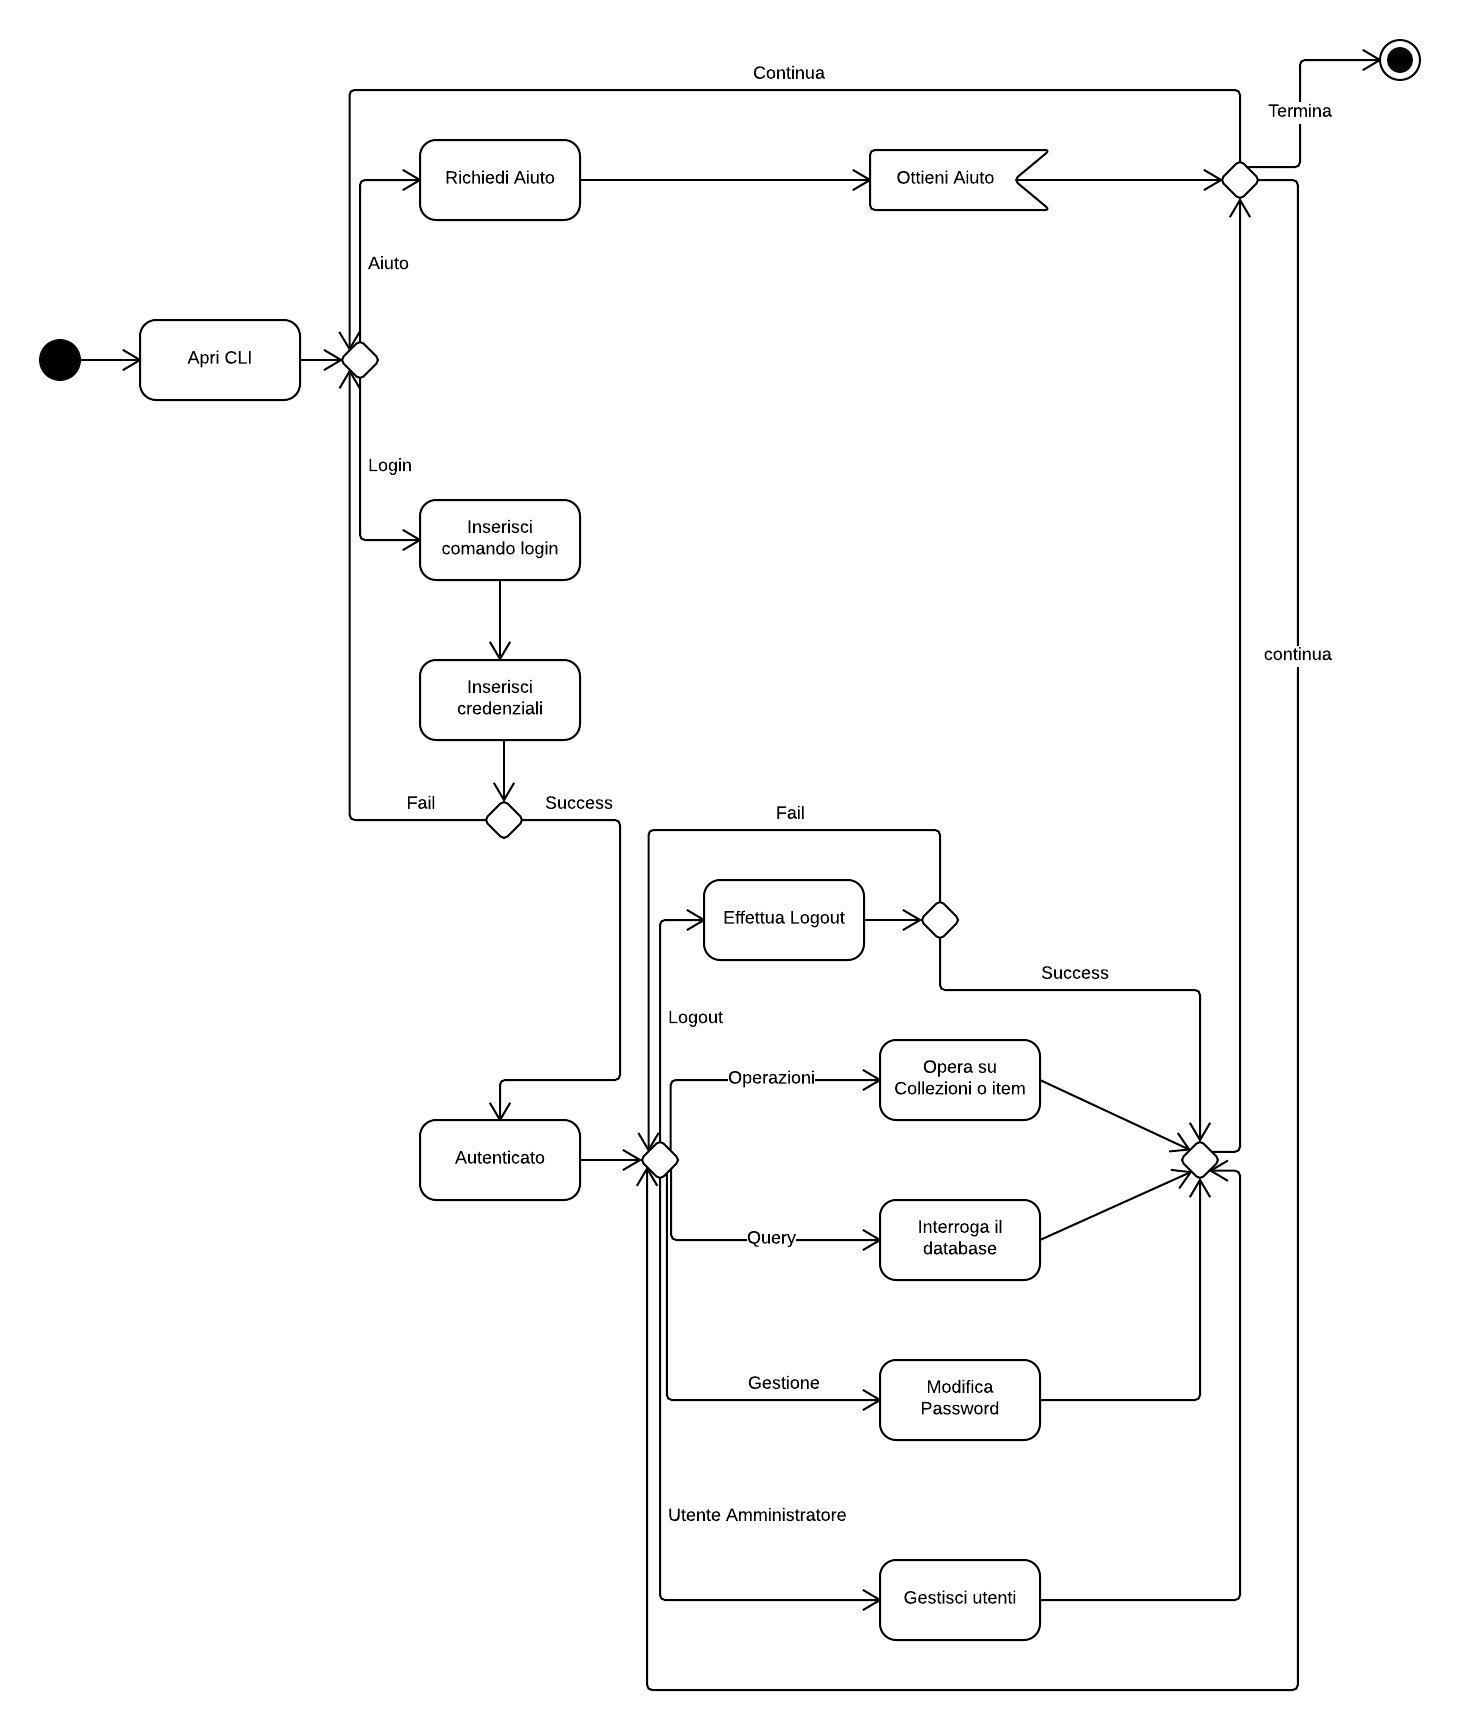
\includegraphics[width=0.8\textwidth, keepaspectratio]{img/diagrammiAttivita/visioneGenerale.jpeg}
    \caption{Diagrammi attività\ -\ Visione generale}
  \end{center}
\end{figure}

\subsection{Operazioni su collezioni e/o item}
\subsubsection{Creazione collezione}

Questo tipo di operazione permette di inserire una collezione all'interno del
database. Come si vede dal grafico che segue, l'utente dovrà inserire il
comando per la creazione della collezione, il nome della collezione stessa e i
suoi parametri. Una volta premuto il tasto invio, l'operazione andrà a buon
termine se l'utente ha scritto correttamente il comando altrimenti verrà
visualizzato un messaggio di errore.

\begin{figure}[H]
  \begin{center}
    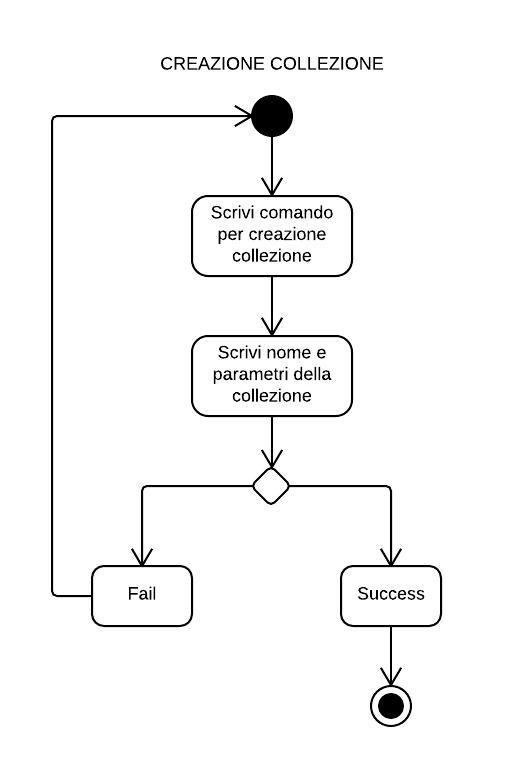
\includegraphics[width=0.3\textwidth, keepaspectratio]{img/diagrammiAttivita/creazioneCollezione.jpeg}
    \caption{Diagrammi attività\ -\ Creazione collezione}
  \end{center}
\end{figure}

\subsubsection{Cancellazione collezione}

Questo tipo di operazione permette di cancellare una collezione dal database.
Come si vede dal grafico che segue, l'utente dovrà inserire il comando per la
cancellazione di una collezione e il nome della collezione stessa. Una volta
premuto il tasto invio, l'operazione andrà a buon termine se l'utente ha
scritto correttamente il comando altrimenti verrà visualizzato un messaggio di
errore.

\begin{figure}[H]
  \begin{center}
    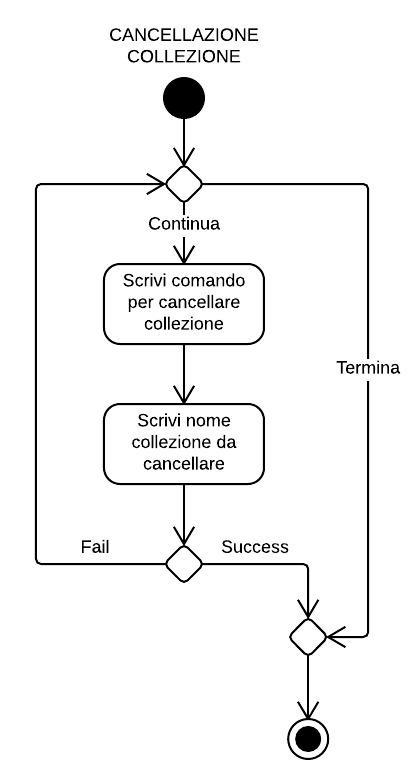
\includegraphics[width=0.3\textwidth, keepaspectratio]{img/diagrammiAttivita/cancCollezione.jpeg}
    \caption{Diagrammi attività\ -\ Cancellazione collezione}
  \end{center}
\end{figure}

\subsubsection{Visualizza collezioni}

Questo tipo di operazione permette di visualizzare le collezioni presenti
all'interno dal database. Come si vede dal grafico che segue, l'utente dovrà
inserire il comando per la visualizzazione delle collezioni. Una volta premuto
il tasto invio, l'operazione andrà a buon termine (ricevendo la lista delle
collezioni) se l'utente ha scritto correttamente il comando altrimenti verrà
visualizzato un messaggio di errore.

\begin{figure}[H]
  \begin{center}
    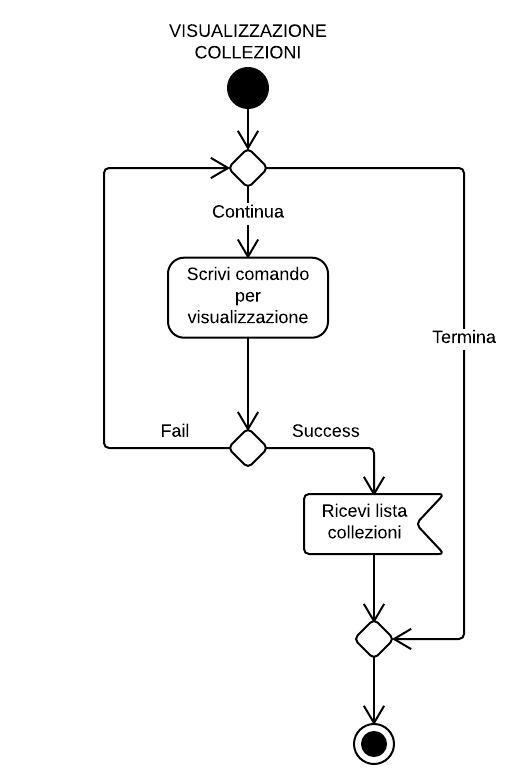
\includegraphics[width=0.3\textwidth, keepaspectratio]{img/diagrammiAttivita/visCollezione.jpeg}
    \caption{Diagrammi attività\ -\ Visualizzazione collezioni}
  \end{center}
\end{figure}

\subsubsection{Modifica nome collezione}

Questo tipo di operazione permette di modificare il nome di una collezione
presente nel database. Come si vede dal grafico che segue, l'utente dovrà
inserire il comando per la rinominazione della collezione, il nome della
collezione stessa e il nuovo nome per essa. Una volta premuto il tasto invio,
l'operazione andrà a buon termine se l'utente ha scritto correttamente il
comando altrimenti verrà visualizzato un messaggio di errore.

\begin{figure}[H]
  \begin{center}
    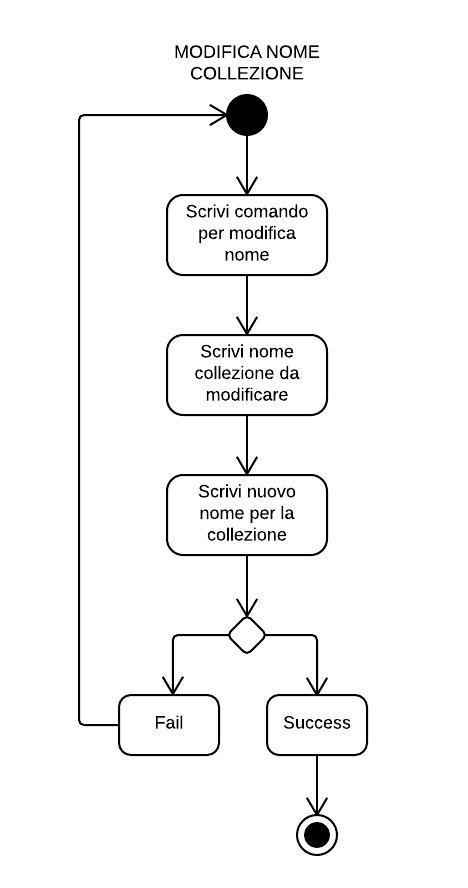
\includegraphics[width=0.3\textwidth, keepaspectratio]{img/diagrammiAttivita/modNomeCollezione.jpeg}
    \caption{Diagrammi attività - Modifica nome collezione}
  \end{center}
\end{figure}

\subsubsection{Inserimento item}

Questo tipo di operazione permette di inserire un item all'interno di una
collezione del database. Come si vede dal grafico che segue, l'utente dovrà
inserire il comando per l'inserimento item, il valore e parametri dell'item
stesso e il nome della collezione dove inserire l'item. Una volta premuto il
tasto invio, l'operazione andrà a buon termine (ricevendo la lista delle
collezioni) se l'utente ha scritto correttamente il comando altrimenti verrà
visualizzato un messaggio di errore.

\begin{figure}[H]
  \begin{center}
    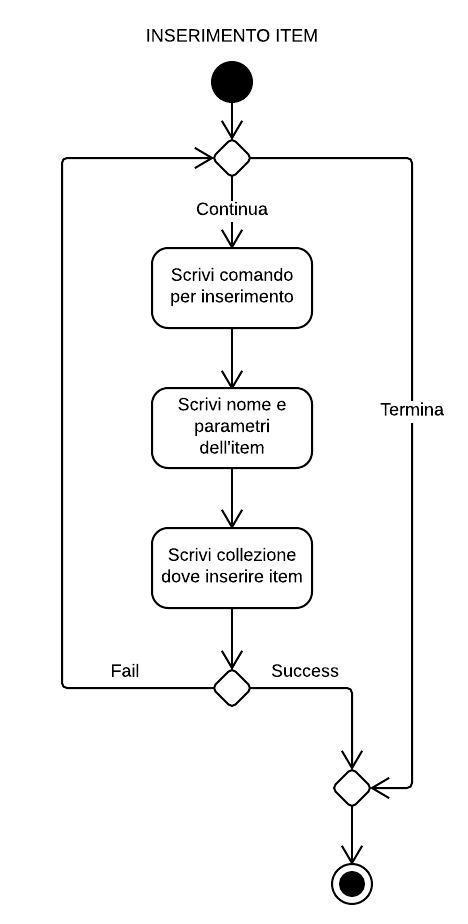
\includegraphics[width=0.3\textwidth, keepaspectratio]{img/diagrammiAttivita/inserimentoItem.jpeg}
    \caption{Diagrammi attività - Inserimento item}
  \end{center}
\end{figure}

\subsubsection{Rimozione item}

Questo tipo di operazione permette di rimuovere un item dall'interno di una
\gloss{collezione} del database. Come si vede dal grafico che segue, l'utente
dovrà inserire il comando per l'eliminazone di un item, il nome della
collezione da dove rimuovere l'item e il nome dell'item stesso. Una volta
premuto il tasto invio, l'operazione andrà a buon termine (ricevendo la lista
delle collezioni) se l'utente ha scritto correttamente il comando altrimenti
verrà visualizzato un messaggio di errore.

\begin{figure}[H]
  \begin{center}
    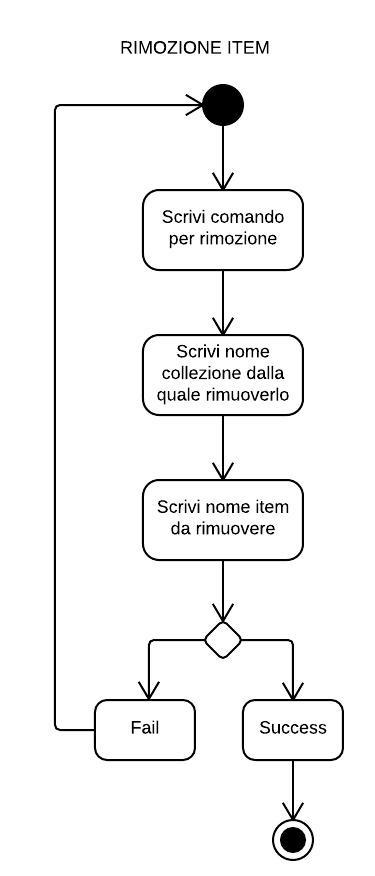
\includegraphics[width=0.3\textwidth, keepaspectratio]{img/diagrammiAttivita/rimozioneItem.jpeg}
    \caption{Diagrammi attività\ -\ Rimozione item}
  \end{center}
\end{figure}

\subsubsection{Aggiunta collaboratore}

Questo tipo di operazione permette di aggiungere un \gloss{collaboratore} ad
una collezione presente nel database. Come si vede dal grafico che segue,
l'utente dovrà inserire il comando per l'aggiunta di un collaboratore ad una
collezione, lo username del collaboratore e il nome della collezione alla
quale aggiungerlo. Una volta premuto il tasto invio, l'operazione andrà a buon
termine se l'utente ha scritto correttamente il comando altrimenti verrà
visualizzato un messaggio di errore.

\begin{figure}[H]
  \begin{center}
    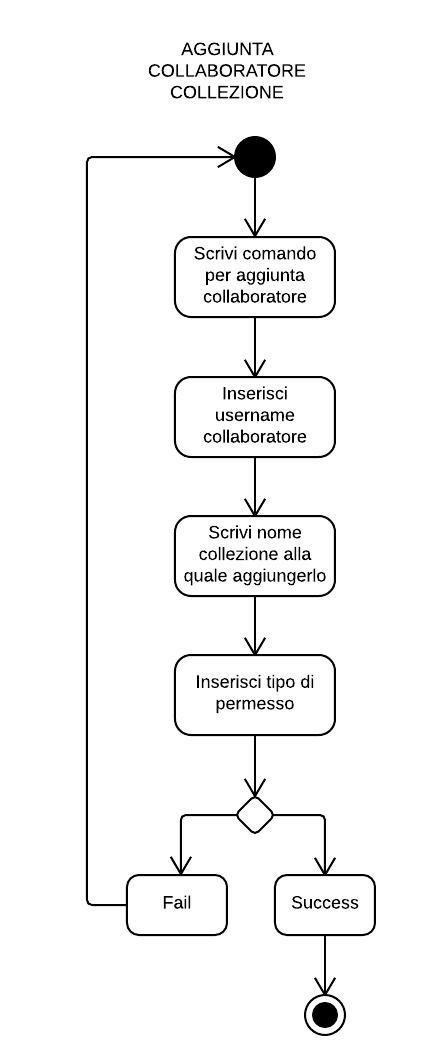
\includegraphics[width=0.3\textwidth, keepaspectratio]{img/diagrammiAttivita/aggCollaboratore.jpeg}
    \caption{Diagrammi attività\ -\ Aggiunta collaboratore}
  \end{center}
\end{figure}

\subsubsection{Rimozione collaboratore}

Questo tipo di operazione permette di rimuovere un collaboratore da una
collezione presente nel database. Come si vede dal grafico che segue, l'utente
dovrà inserire il comando per la rimozione di un collaboratore da una
collezione, lo username del collaboratore e il nome della collezione dalla
quale rimuoverlo. Una volta premuto il tasto invio, l'operazione andrà a buon
termine se l'utente ha scritto correttamente il comando altrimenti verrà
visualizzato un messaggio di errore.

\begin{figure}[H]
  \begin{center}
    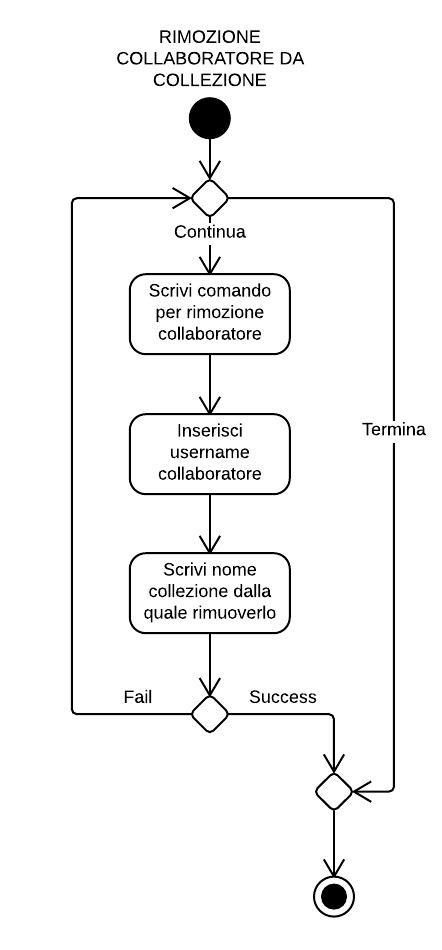
\includegraphics[width=0.3\textwidth, keepaspectratio]{img/diagrammiAttivita/rimozioneCollaboratore.jpeg}
    \caption{Diagrammi attività\ -\ Rimozione collaboratore}
  \end{center}
\end{figure}

\subsubsection{Import}

Questo tipo di operazione permette di importare nel database collezioni o item
tramite file \gloss{JSON}. Come si vede dal grafico che segue, l'utente dovrà
inserire il comando per l'importazione e il path che porta al file desiderato.
Una volta premuto il tasto invio, l'operazione andrà a buon termine se
l'utente ha scritto correttamente il comando altrimenti verrà visualizzato un
messaggio di errore.

\begin{figure}[H]
  \begin{center}
    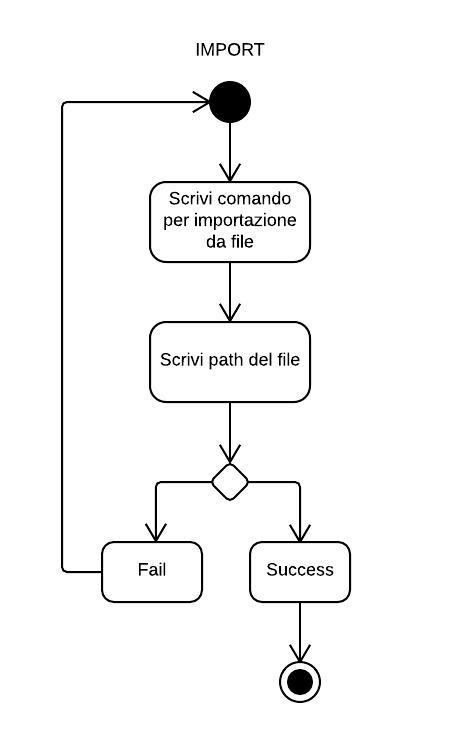
\includegraphics[width=0.3\textwidth, keepaspectratio]{img/diagrammiAttivita/import.jpeg}
    \caption{Diagrammi attività - Import}
  \end{center}
\end{figure}

\subsection{Interrogazione del database}

Questo tipo di operazione permette di interrogare il database tramite delle
query. Come si vede dal grafico che segue, l'utente dovrà inserire il comando
per l'interrogazione del database e i parametri per la ricerca. Una volta
premuto il tasto invio, l'operazione andrà a buon termine se l'utente ha
scritto correttamente il comando, ricevendo il risultato della query,
altrimenti verrà visualizzato un messaggio di errore.

\begin{figure}[H]
  \begin{center}
    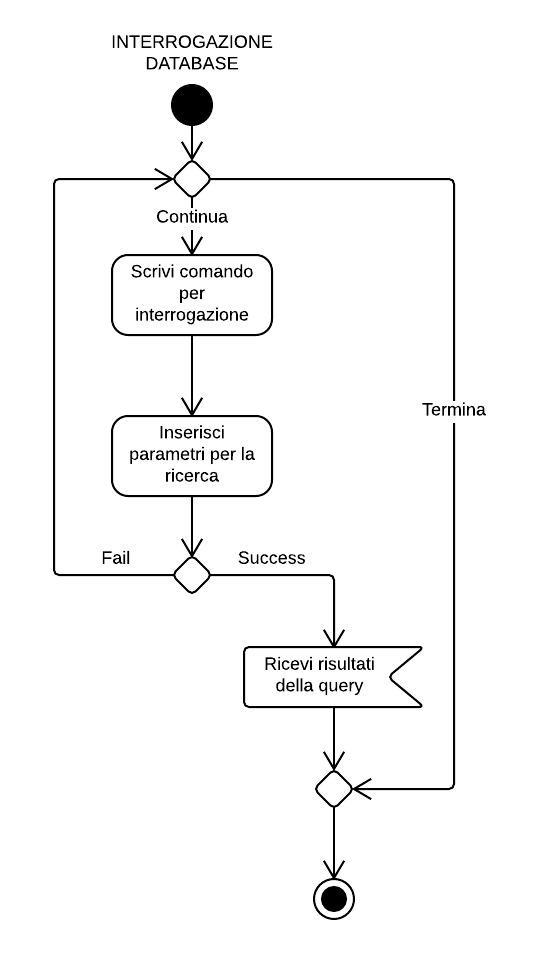
\includegraphics[width=0.3\textwidth, keepaspectratio]{img/diagrammiAttivita/query.jpeg}
    \caption{Diagrammi attività - Interrogazione del database}
  \end{center}
\end{figure}

\subsection{Modifica password}

Questo tipo di operazione permette di modificare la propria password. Come si
vede dal grafico che segue, l'utente dovrà inserire il comando per la modifica
della password, la vecchia password, la nuova password e confermare
quest'ultima. Una volta premuto il tasto invio, l'operazione andrà a buon
termine se l'utente ha scritto correttamente il comando altrimenti verrà
visualizzato un messaggio di errore.

\begin{figure}[H]
  \begin{center}
    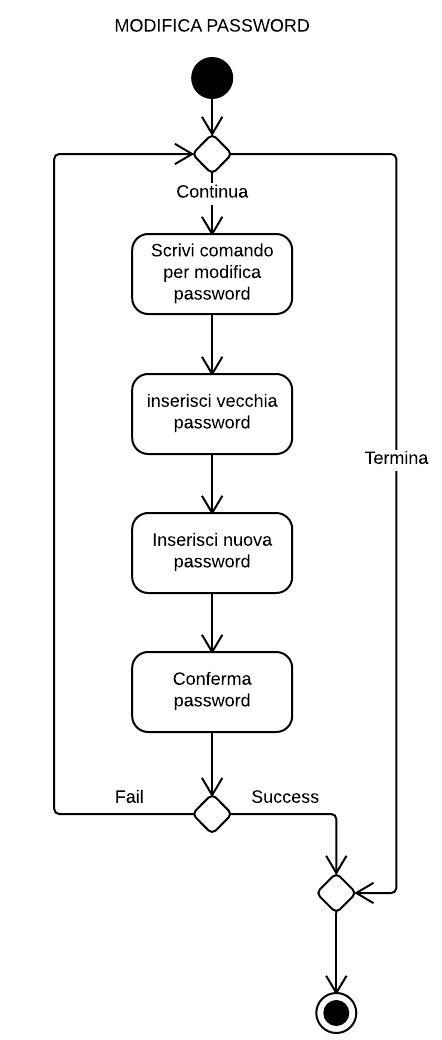
\includegraphics[width=0.3\textwidth, keepaspectratio]{img/diagrammiAttivita/modificaPsw.jpeg}
    \caption{Diagrammi attività - Modifica password}
  \end{center}
\end{figure}

\subsection{Gestione utenti}

La gestione utenti, possibile solo ad un utente amministratore, prevede la
possibilità di aggiungere o rimuovere un utente dal database e la possibilità
di resettare la password di un utente. Per aggiungere o rimuovere un utente,
l'amministratore dovrà inserire il rispettivo comando, lo username dell'utente
da aggiungere/rimuovere dal database e una conferma. Per resettare la password
di un utente, l'amministratore dovrà scrivere il comando per il reset della
password, lo username dell'utente interessato e una conferma. Una volta
premuto il tasto invio, le operazione andranno a buon termine se l'utente ha
scritto correttamente il comando altrimenti verrà visualizzato un messaggio di
errore.

\begin{figure}[H]
  \begin{center}
    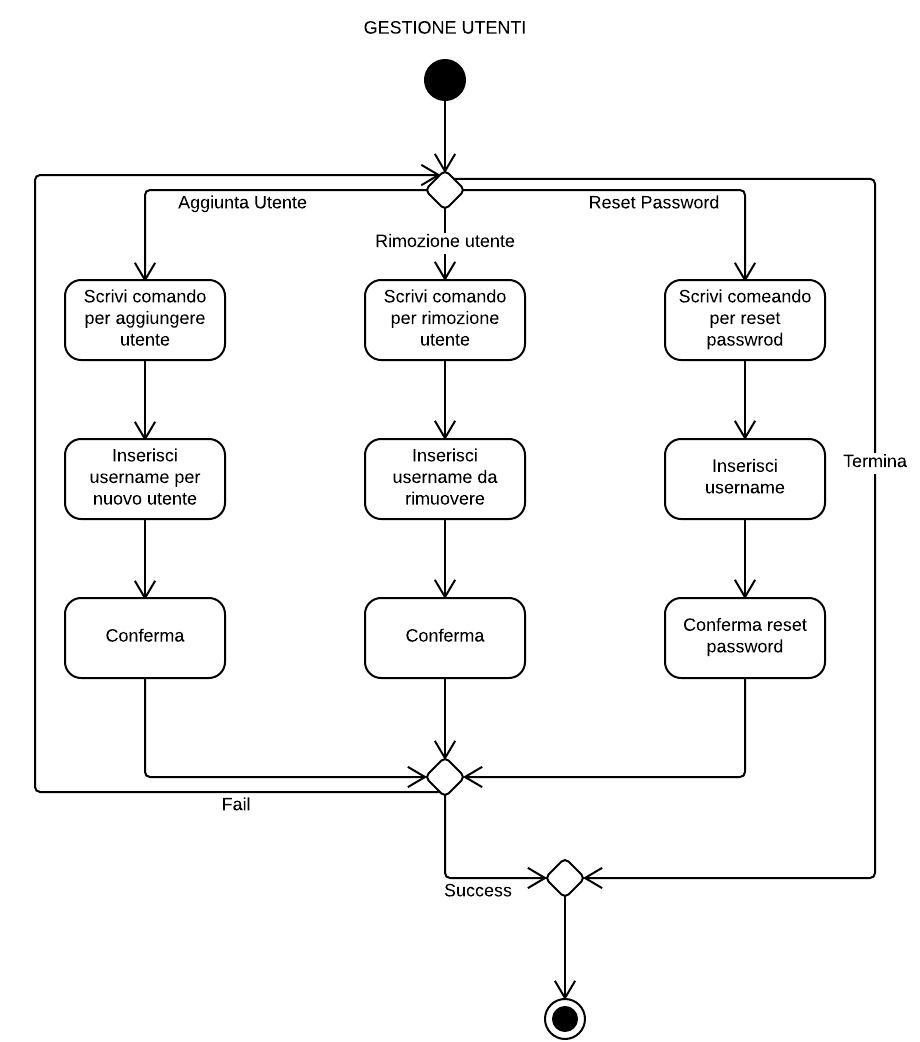
\includegraphics[width=0.6\textwidth, keepaspectratio]{img/diagrammiAttivita/gestioneUtenti.jpeg}
    \caption{Diagrammi attività - Gestione utenti}
  \end{center}
\end{figure}

\section{Diagrammi di Sequenza}

In questa sezione, vengono illustrati i diagrammi di sequenza che descrivono
le interazioni tra le varie componenti del sistema e in particolare lo scambio
di messaggi che avviene tra gli attori nella componente server di actorbase.\\
Sono stati creati dai \textit{Progettisti} diversi diagrammi con diversi livelli
di astrazione.\\
Per semplificare i diagrammi, evitare ripetitività e migliorare la leggibilità di
questi, nella maggior parte dei seguenti l'input sarà dato dalla componente \gloss{Driver}. In un utilizzo reale sarà un utente che utilizza il \gloss{Driver} o la
\gloss{CLI} che darà l'input iniziale.

\subsection{Interazioni generali tra componenti}
Questo diagramma rappresenta l'interazione generale tra le tre componenti che
compongono il sistema actorbase.\\
L'utente è connesso alla \gloss{CLI} e inserisce un comando. A questo punto la componente \gloss{CLI} (se non è instanziato un \gloss{Driver} lo crea per poi utilizzarlo) utilizza il \gloss{Driver} per richiamare il metodo relativo al comando inserito dall'utente.\\Il \gloss{Driver} provvederà a tradurre il comando coi relativi parametri immessi dall'utente in una stringa RESP e la invierà al server attraverso un \gloss{socket tcp}.\\ %TODO linkare RESP
Il server provvederà a fare le elaborazioni richieste attraverso l'uso degli attori
e quando queste saranno finite risponderà al \gloss{Driver} mandando via \gloss{socket tcp} una string RESP che a sua volta provvederà a trasformarla in un
\hyperref[sec:driver::actorbasedata::actorbaseobject]{actorbase object} e lo restituirà al suo utilizzatore.\\ %TODO linkare RESP
\begin{figure}[H]
  \begin{center}
    \includegraphics[width=0.9\textwidth, keepaspectratio]{img/diagrammiSequenza/ScambioMessaggiGenerico.png}
    \caption{Diagramma di sequenza - Interazioni generali tra componenti}
  \end{center}
\end{figure}

\subsection{Inserimento di un Item}

Questo diagramma rappresenta l'interazione tra le componenti nel caso di una richiesta di inserimento di un \gloss{item}.\\
La componente \hyperref[sec:actorbase::driver::client::Connection]{actorbase::driver::client::Connection}
manda tramite \gloss{socket tcp} al \hyperref[sec:actorbase::actorsystem::clientactor::ClientActor]{actorbase::actorsystem::clientactor::ClientActor}
una string RESP contenente il comando di inserimento \gloss{item} con
i parametri.\\ %TODO linkare RESP
Da questo componente parte il messaggio di Insert(key, value) ad un \hyperref[sec:actorbase::actorsystem::clientactor::MainActor]{actorbase::actorsystem::clientactor::MainActor} scelto in base ad una
politica di \gloss{routing}. Il MainActor manderà un messaggio allo \hyperref[sec:actorbase::actorsystem::clientactor::StoreFinder]{actorbase::actorsystem::clientactor::StoreFinder} relativo il quale manderà un messaggio allo \hyperref[sec:actorbase::actorsystem::clientactor::StoreKeeper]{actorbase::actorsystem::clientactor::StoreKeeper} che dovrà salvarsi l'informazione
sulla propria mappa.\\
A questo punto lo StoreKeeper manderà un messaggio al ClientActor con la risposta
(positiva o negativa che sia) il quale risponderà sempre tramite \gloss{socket tcp} al \gloss{Driver} con una stringa RESP.
\begin{figure}[H]
  \begin{center}
    \includegraphics[width=0.9\textwidth, keepaspectratio]{img/diagrammiSequenza/esempioInsert.png}
    \caption{Diagramma di sequenza - Inserimento di un item}
  \end{center}
\end{figure}

\subsection{Inserimento di un Item con StoreKeeper pieno}

Questo diagramma rappresenta l'interazione tra le componenti nel caso di una richiesta di inserimento di un \gloss{item} in uno StoreKeeper con una mappa piena.\\
La componente \hyperref[sec:actorbase::driver::client::Connection]{actorbase::driver::client::Connection}
manda tramite \gloss{socket tcp} al \hyperref[sec:actorbase::actorsystem::clientactor::ClientActor]{actorbase::actorsystem::clientactor::ClientActor}
una string RESP contenente il comando di inserimento \gloss{item} con
i parametri.\\ %TODO linkare RESP
Da questo componente parte il messaggio di Insert(key, value) ad un \hyperref[sec:actorbase::actorsystem::clientactor::MainActor]{actorbase::actorsystem::clientactor::MainActor} scelto in base ad una
politica di \gloss{routing}. Il MainActor manderà un messaggio allo \hyperref[sec:actorbase::actorsystem::clientactor::StoreFinder]{actorbase::actorsystem::clientactor::StoreFinder} relativo il quale manderà un messaggio allo \hyperref[sec:actorbase::actorsystem::clientactor::StoreKeeper]{actorbase::actorsystem::clientactor::StoreKeeper} che essendo pieno manda un
messaggio DuplicateRequestSK contenente metà della propria mappa e una ActorRef del proprio parent ad un \hyperref[sec:actorbase::actorsystem::clientactor::Manager]{actorbase::actorsystem::clientactor::Manager}. Il Manager inoltra il messaggio DuplicateRequestSK al parent dello StoreKeeper precedentemente coinvolto. Questo StoreFinder infine creerà un nuovo Storekeeper con il pezzo di mappa ricevuto. \\
A questo punto il nuovo StoreKeeper manderà un messaggio al ClientActor con
la risposta (positiva o negativa che sia) il quale risponderà sempre tramite
\gloss{socket tcp} al \gloss{Driver} con una stringa RESP.
\begin{figure}[H]
  \begin{center}
    \includegraphics[width=0.9\textwidth, keepaspectratio]{img/diagrammiSequenza/esempioInsert.png}
    \caption{Diagramma di sequenza - Inserimento di un item}
  \end{center}
\end{figure}

\subsection{Autenticazione}

Questo diagramma rappresenta l'interazione tra le componenti nel caso di una richiesta di autenticazione di un utente.\\
La componente \hyperref[sec:actorbase::driver::client::Connection]{actorbase::driver::client::Connection}
manda tramite \gloss{socket tcp} al \hyperref[sec:actorbase::actorsystem::clientactor::ClientActor]{actorbase::actorsystem::clientactor::ClientActor}
una string RESP contenente il comando di inserimento \gloss{item} con
i parametri.\\ %TODO linkare RESP
Da questo componente parte il messaggio di GetItemFrom(UsersCollection, Username) ad un \hyperref[sec:actorbase::actorsystem::clientactor::MainActor]{actorbase::actorsystem::clientactor::MainActor} scelto in base ad una
politica di \gloss{routing}. Il MainActor manderà un messaggio allo \hyperref[sec:actorbase::actorsystem::clientactor::StoreFinder]{actorbase::actorsystem::clientactor::StoreFinder} relativo il quale manderà un messaggio getPassword(username) allo \hyperref[sec:actorbase::actorsystem::clientactor::UserKeeper]{actorbase::actorsystem::clientactor::UserKeeper}. Quest'ultimo risponderà al ClientActor con un messaggio loginResponse contenente la password relativa allo username richiesto.\\
Il ClientActor eseguirà un confronto tra la password immessa dall'utente e la password ritornata dallo UserKeeper. In caso positivo cambierà il proprio stato
e risponderà al \gloss{Driver} con un messaggio che indica un esito positivo. In caso negativo resterà nello stato attuale e manderà un messaggio al \gloss{Driver} che indica un esito negativo.
\begin{figure}[H]
  \begin{center}
    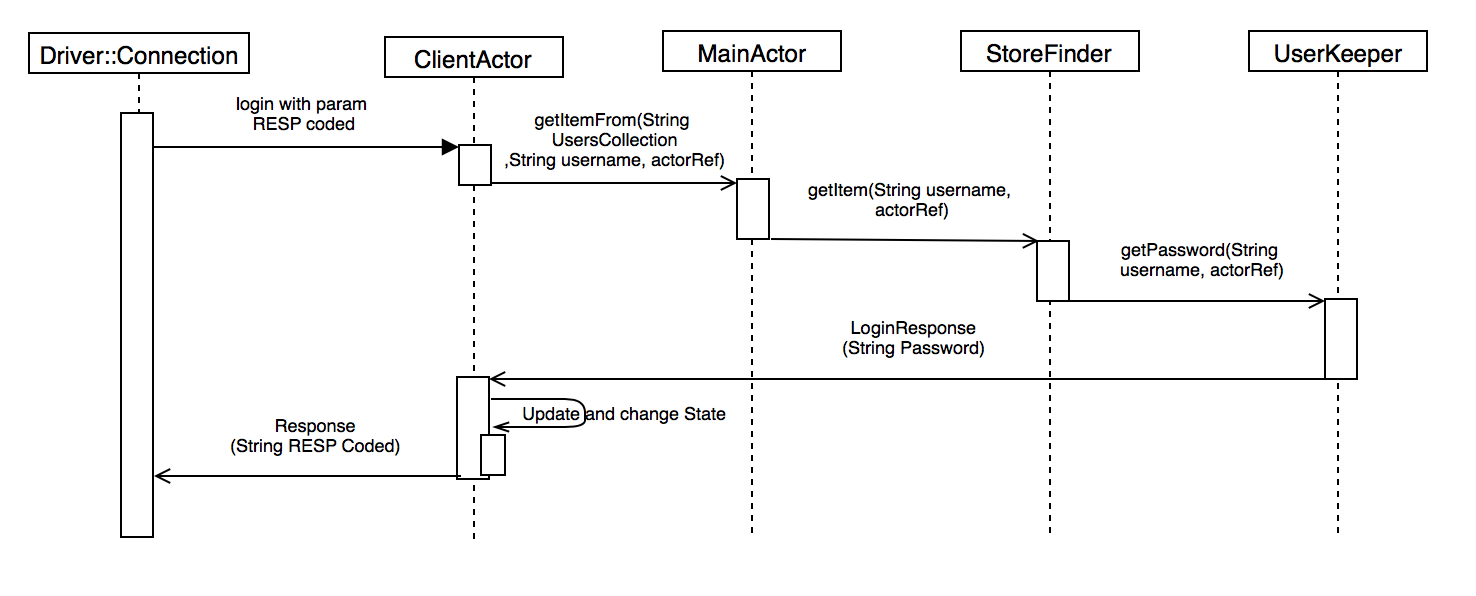
\includegraphics[width=0.9\textwidth, keepaspectratio]{img/diagrammiSequenza/esempioAuth.png}
    \caption{Diagramma di sequenza - Autenticazione}
  \end{center}
\end{figure}

\subsection{Salvataggio su filesystem}

Questo diagramma rappresenta l'interazione tra le componenti nel caso venga
effettuato un salvataggio dei dati su filesystem.\\
La componente \hyperref[sec:actorbase::driver::client::Connection]{actorbase::driver::client::Connection}
manda tramite \gloss{socket tcp} al \hyperref[sec:actorbase::actorsystem::clientactor::ClientActor]{actorbase::actorsystem::clientactor::ClientActor}
una string RESP contenente il comando di inserimento \gloss{item} con
i parametri.\\ %TODO linkare RESP
Da questo componente parte il messaggio di Insert(key, value) ad un \hyperref[sec:actorbase::actorsystem::clientactor::MainActor]{actorbase::actorsystem::clientactor::MainActor} scelto in base ad una
politica di \gloss{routing}. Il MainActor manderà un messaggio allo \hyperref[sec:actorbase::actorsystem::clientactor::StoreFinder]{actorbase::actorsystem::clientactor::StoreFinder} relativo il quale manderà un messaggio allo \hyperref[sec:actorbase::actorsystem::clientactor::StoreKeeper]{actorbase::actorsystem::clientactor::StoreKeeper} che dovrà salvarsi l'informazione
sulla propria mappa.\\
A questo punto lo StoreKeeper manderà un messaggio al Warehouseman di tipo Save e
successivamente manderà un messaggio al ClientActor con la risposta
(positiva o negativa che sia) il quale risponderà sempre tramite \gloss{socket tcp} al \gloss{Driver} con una stringa RESP.
Nel frattempo l'attore di tipo Warehouseman eseguirà un salvataggio su disco dei propri dati previa serializzazione.\\
Si noti che la frequenza con cui gli attori di tipo Warehousename eseguiranno
l'aggiornamento delle proprie strutture dati e il salvataggio sarà specificata
tramite un parametro di configurazione del sistema.\\
\begin{figure}[H]
  \begin{center}
    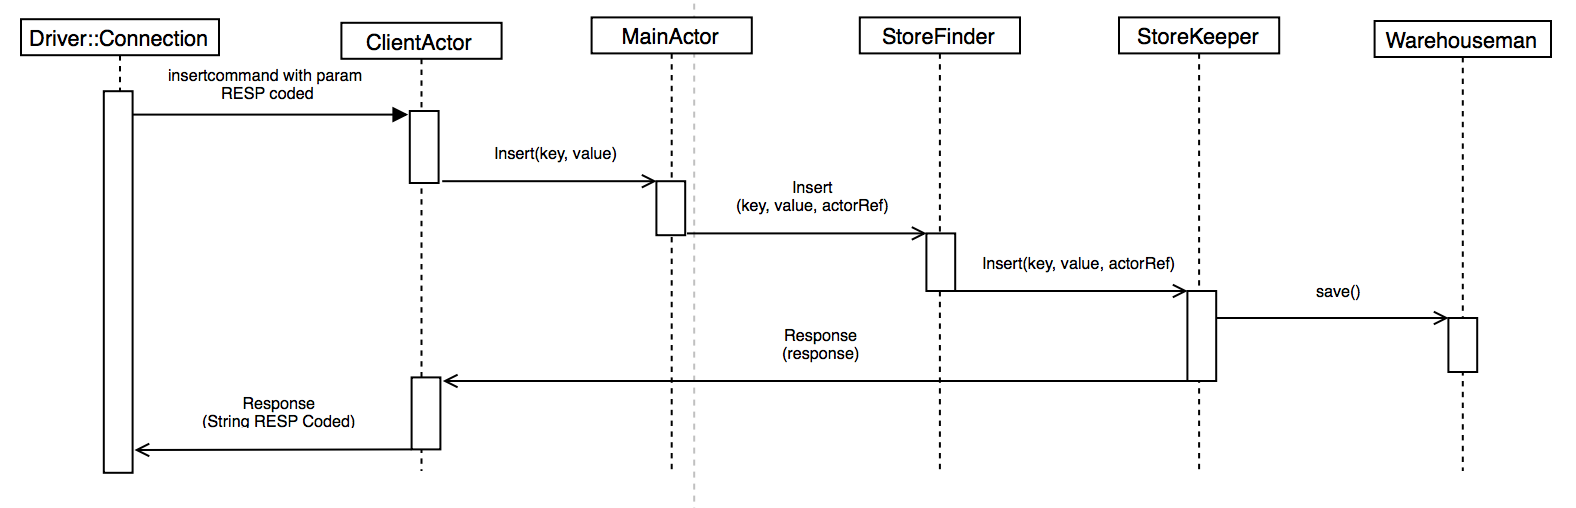
\includegraphics[width=0.9\textwidth, keepaspectratio]{img/diagrammiSequenza/esempioSave.png}
    \caption{Diagramma di sequenza - Inserimento di un item}
  \end{center}
\end{figure}

\subsection{Aggiornamento di un attore ninja}

Questo diagramma rappresenta l'interazione tra le componenti nel caso venga
effettuato un aggiornamento dei dati su un attore Ninja.\\
La componente \hyperref[sec:actorbase::driver::client::Connection]{actorbase::driver::client::Connection}
manda tramite \gloss{socket tcp} al \hyperref[sec:actorbase::actorsystem::clientactor::ClientActor]{actorbase::actorsystem::clientactor::ClientActor}
una string RESP contenente il comando di inserimento \gloss{item} con
i parametri.\\ %TODO linkare RESP
Da questo componente parte il messaggio di Insert(key, value) ad un \hyperref[sec:actorbase::actorsystem::clientactor::MainActor]{actorbase::actorsystem::clientactor::MainActor} scelto in base ad una
politica di \gloss{routing}. Il MainActor manderà un messaggio allo \hyperref[sec:actorbase::actorsystem::clientactor::StoreFinder]{actorbase::actorsystem::clientactor::StoreFinder} relativo il quale manderà un messaggio allo \hyperref[sec:actorbase::actorsystem::clientactor::StoreKeeper]{actorbase::actorsystem::clientactor::StoreKeeper} che dovrà salvarsi l'informazione
sulla propria mappa.\\
A questo punto lo StoreKeeper manderà un messaggio al Ninja di tipo Update contenente la struttura dati aggiornata e successivamente manderà un
messaggio al ClientActor con la risposta (positiva o negativa che sia)
il quale risponderà sempre tramite \gloss{socket tcp} al \gloss{Driver} con
una stringa RESP.
Nel frattempo l'attore di tipo Ninja eseguirà un aggiornamento della propria struttura dati.\\
Si noti che la frequenza di aggiornamento degli attori di tipo ninja sarà
specificata tramite un parametro di configurazione del sistema.
\begin{figure}[H]
  \begin{center}
    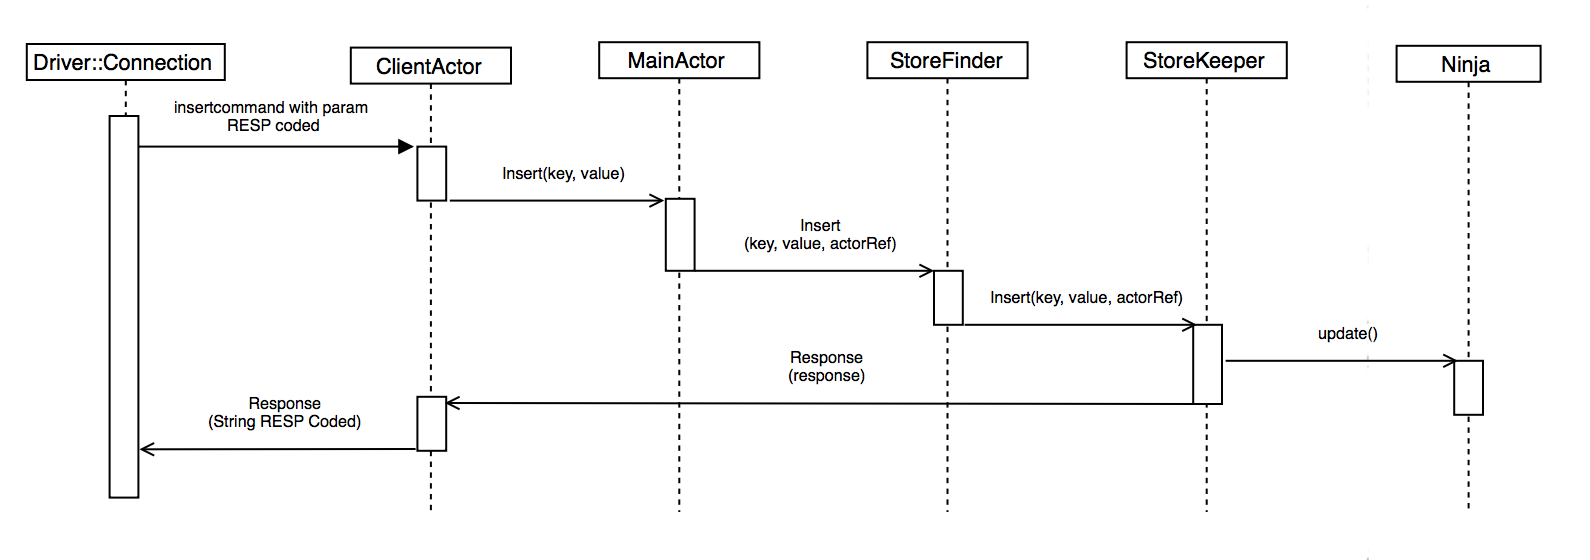
\includegraphics[width=0.9\textwidth, keepaspectratio]{img/diagrammiSequenza/esempioNinja.png}
    \caption{Diagramma di sequenza - Aggiornamento di un attore ninja}
  \end{center}
\end{figure}

\subsection{Aggiunta collaboratore (in sola lettura)}

Questo diagramma rappresenta l'interazione tra le componenti nel caso di una richiesta di autenticazione di un utente.\\
La componente \hyperref[sec:actorbase::driver::client::Connection]{actorbase::driver::client::Connection}
manda tramite \gloss{socket tcp} al \hyperref[sec:actorbase::actorsystem::clientactor::ClientActor]{actorbase::actorsystem::clientactor::ClientActor}
una string RESP contenente il comando di aggiunta collaboratore \gloss{item} con
i parametri.\\ %TODO linkare RESP
Da questo componente parte il messaggio di addCollaborator(collection, permission, username) ad un \hyperref[sec:actorbase::actorsystem::clientactor::MainActor]{actorbase::actorsystem::clientactor::MainActor} scelto in base ad una
politica di \gloss{routing}. Il MainActor manderà un messaggio allo
\hyperref[sec:actorbase::actorsystem::clientactor::StoreFinder]{actorbase::actorsystem::clientactor::StoreFinder}
relativo il quale manderà un messaggio addReadCollection(collection) allo
\hyperref[sec:actorbase::actorsystem::clientactor::UserKeeper]{actorbase::actorsystem::clientactor::UserKeeper}.
Quest'ultimo dovrà aggiungere alla mappa delle collezioni di cui l'utente
relativo ha accesso in sola lettura la collezione inviatagli.
Poi manderà al ClientActor un messaggio UpdateReadCollections(collection)
contenente la collezione da aggiungere.\\
Il ClientActor effettuerà l'aggiornamento e risponderà al \gloss{Driver}
con un messaggio che indica un esito positivo. In caso negativo resterà nello
stato attuale e manderà un messaggio al \gloss{Driver} che indica un esito
negativo.\\
Nel caso di aggiunta di un collaboratore con permessi di lettura e scrittura
l'interazione tra gli attori è la stessa con differenza di qualche messaggio
specifico.\\
\begin{figure}[H]
  \begin{center}
    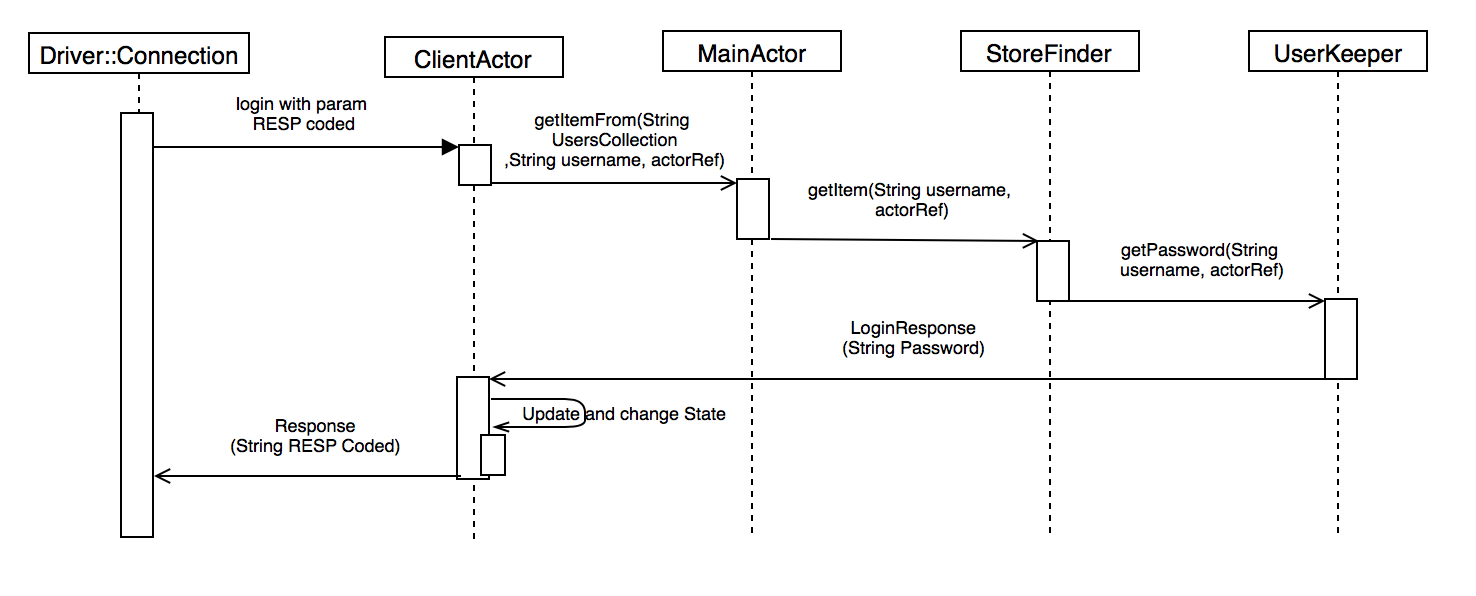
\includegraphics[width=0.9\textwidth, keepaspectratio]{img/diagrammiSequenza/esempioAuth.png}
    \caption{Diagramma di sequenza - Autenticazione}
  \end{center}
\end{figure}

\subsection{Connessione al server tramite Driver}

Questo diagramma rappresenta l'interazione tra le componenti nel caso di una richiesta di connessione al server di un utente tramite uso del \gloss{Driver}.\\Si noti che tramite utilizzo della \gloss{CLI} il diagramma sarebbe lo stesso con l'aggiunta della componente \gloss{CLI}.\\
L'utente crea un oggetto di tipo \hyperref[sec:actorbase::driver::client::ActorbaseClient]{actorbase::driver::client::ActorbaseClient}
il quale crea a sua volta un oggetto di tipo \hyperref[sec:actorbase::driver::client::Connection]{actorbase::driver::client::Connection}.
\hyperref[sec:actorbase::driver::client::Connection]{actorbase::driver::client::Connection}
instaura una connessione \gloss{tcp} con la componente
\hyperref[sec:actorbase::actorsystem::tcpserver::TCPServer]{actorbase::actorsystem::tcpserver::TCPServer} la quale crea un attore di tipo
\hyperref[sec:actorbase::actorsystem::clientactor::ClientActor]{actorbase::actorsystem::clientactor::ClientActor}
per gestire l'interazione tra \gloss{Driver} e server. A creazione avvenuta risponde al \gloss{Driver} il quale a cascata informa l'utente dell'avvenuta
connessione.\\
Dal diagramma possiamo vedere che le richieste successivamente inserite
dall'utente verranno gestite dal proprio ClientActor.\\
\begin{figure}[H]
  \begin{center}
    \includegraphics[width=0.9\textwidth, keepaspectratio]{img/diagrammiSequenza/esempioConnessione.png}
    \caption{Diagramma di sequenza - Connessione al server}
  \end{center}
\end{figure}

\section{Design Pattern}

I \gloss{Design Pattern} rappresentano soluzioni progettuali generali ad un
problema ricorrente. Si tratta di  modelli logici da applicare per la
risoluzione di un problema ancor prima della definizione dell'algoritmo
risolutivo vero e proprio, favoriscono il riutilizzo del codice e rendono
l'architettura più manutenibile.\\
I \gloss{Design Pattern} possono essere suddivisi in:

\begin{itemize}
\item \textbf{architetturali:} operano al livello più alto,
  esprimono schemi di base per impostare l'organizzazione strutturale di un
  sistema software;
\item \textbf{creazionali:} nascondono i costruttori delle classi e mettono dei
  metodi al loro posto creando un'interfaccia, in questo modo forniscono
  un'astrazione del processo di instanziazione degli oggetti;
\item \textbf{strutturali:} consentono di riutilizzare degli oggetti esistenti
  fornendo agli utilizzatori un'interfaccia più adatta alle loro esigenze;
\item \textbf{comportamentali:} definiscono soluzioni per le interazioni tra
  oggetti.
\end{itemize}

Si rimanda all'Appendice A per un approfondimento dei \gloss{Design Pattern}
utilizzati nel progetto \textbf{Actorbase}.

\subsection{Design Pattern Architetturali}

\subsubsection{MVC}

\begin{itemize}
\item \textbf{Scopo:} E' stato scelto l'utilizzo del pattern \gloss{Model}
  \gloss{View} \gloss{Controller} (\gloss{MVC}) per l'alto grado di separazione
  tra la parte logica dell'applicazione e parte grafica che offre;
\item \textbf{Utilizzo:} Viene utilizzato per delineare l'architettura generale
  della componente \gloss{CLI} (Command Line Interface) del progetto. La parte
  \gloss{View} funge da interfaccia con l'utente, si occupa di leggere l'input e
  inviarlo al Controller, il quale si occupa di validare l'input
  e inviare il comando estrapolato al \gloss{Model}.\\
  Il \gloss{Model} mediante un \gloss{Command Pattern} (vedi~\hyperref[sec:CommandPattern]{Command Pattern})
  esegue il comando richiesto e notifica la \gloss{View} utilizzando un \gloss{Observer Pattern}
  (vedi~\hyperref[sec:ObserverPattern]{Observer Pattern}) secondo la variante \gloss{Push model}.
\end{itemize}

\subsection{Design Pattern Creazionali}

\subsubsection{Singleton}

\begin{itemize}
\item \textbf{Scopo:} Viene utilizzato per le classi di cui è preferibile avere un'unica istanza
  durante l'esecuzione dell'applicazione;
\item \textbf{Utilizzo:} E' stato utilizzato una sola volta per la classe di connessione all'interno
  della componente \gloss{driver}, in modo da offrire un unico punto di accesso al server.
\end{itemize}

\subsection{Design Pattern Strutturali}

\subsubsection{Facade}

\begin{itemize}
\item \textbf{Scopo:} Il pattern \gloss{Facade} viene usato per fornire
  un'interfaccia unica e semplificata a più classi;
\item \textbf{Utilizzo:} Viene utilizzato all'interno della componente
  \gloss{driver} per l'esecuzione e l'invio al server dei comandi mediante
  la classe CommandRunner, la quale mediante l'istanza \gloss{Singleton} di
  Connection invia e riceve i comandi al server.
\end{itemize}

\subsection{Design Pattern Comportamentali}

\subsubsection{Command Pattern}

\label{sec:CommandPattern}

\begin{itemize}
\item \textbf{Scopo:} Viene utilizzato per separare l'implementazione di un'azione
  (\gloss{Receiver}) dal richiamante dell'azione stessa (\gloss{Invoker}).
\item \textbf{Utilizzo:} Viene utilizzato per la gestione dei comandi nella componente
  \gloss{CLI}, e funge da \gloss{Model} dell'architettura \gloss{MVC} utilizzata.\\
  Le classi che implementano i comandi realizzando l'interfaccia \verb=Command= sono:
  \begin{itemize}
  \item \verb=FindCommand=
  \item \verb=ListCommand=
  \item \verb=LoginCommand=
  \item \verb=LogoutCommand=
  \item \verb=HelpCommand=
  \item \verb=InsertItemCommand=
  \item \verb=RemoveItemCommand=
  \item \verb=RenameCollectionCommand=
  \item \verb=CreateCollectionCommand=
  \item \verb=RemoveCollectionCommand=
  \item \verb=ImportCommand=
  \item \verb=ExportCommand=
  \item \verb=AddContributorCommand=
  \item \verb=RemoveContributorCommand=
  \item \verb=ResetPasswordCommand=
  \item \verb=AddUserCommand=
  \item \verb=RemoveUserCommand=
  \end{itemize}
\end{itemize}

La classe incaricata di eseguire i comandi è \verb=CommandReceiver=, invocata mediante
\verb=CommandInvoker=, utilizzando i parametri ricevuti dalla parte \gloss{Controller}
dell'architettura \gloss{MVC} scelta per la componente \gloss{CLI}.

\subsubsection{Iterator Pattern}

\begin{itemize}
\item \textbf{Scopo:} Fornisce un sistema di navigazione attraverso gli elementi di una generica struttura dati contenitrice,
  senza esporre i dettagli dell'implementazione e della struttura interna del contenitore.
\item \textbf{Utilizzo:} Viene utilizzato nella componente \gloss{driver}, più specificamente nel \gloss{package} \verb=actorbaseobject=
  per permettere l'iterazione degli oggetti restituiti dalla componente \verb=actorsystem=.\\
  Le classi che implementano l'interfaccia \verb=cursor= sono:
  \begin{itemize}
  \item \verb=CollectionCursor=
  \item \verb=ItemCursor=
  \end{itemize}
\end{itemize}

\subsubsection{Observer Pattern}

\label{sec:ObserverPattern}

\begin{itemize}
\item \textbf{Scopo:} Viene utilizzato per tenere sotto controllo lo stato di diversi oggetti, ed è parte dell'implementazione
  del \gloss{Design Pattern} \gloss{MVC} con logica \gloss{push model}, il funzionamento si basa su meccanismi di callback.
\item \textbf{Utilizzo:} E' stato utilizzato nella componente \gloss{CLI} del progetto in modo da ottenere una \gloss{view}
  auto-aggiornante sull'output prodotto dai comandi inviati alla componente \gloss{driver}.\\
  Più in dettaglio, la classe \verb=CommandInvoker= realizza l'interfaccia \verb=Observable= aggiungendo l'oggetto di tipo
  \verb=ResultView= alla propria lista di \gloss{observers}, all'esecuzione di ogni comando, notifica \verb=resultview=
  con l'output prodotto.
\end{itemize}

\subsubsection{Strategy}

\begin{itemize}
\item \textbf{Scopo:} Viene usato per isolare più algoritmi all'interno di oggetti e
  ne permette la modifica dinamica.
\item \textbf{Utilizzo:} Nella componente \verb=actorsystem= è stato utilizzato
  per offrire più possibilità di serializzazione e deserializzazione sia in
  ambito di persistenza su disco che in ambito comunicazioni tra server ed
  esterno.\\ Nella componente \gloss{driver} viene offerta una singola
  strategia, dedicata esclusivamente alla comunicazione con la componente
  \verb=actorsystem=, con la scelta di mantenere il \gloss{Design Pattern} in
  vista di eventuali estensioni. Contesti di utilizzo:
  \begin{itemize}

  \item \textbf{driver:}
    \begin{itemize}
    \item Dopo che la classe \verb=Connection= riceve i parametri da inviare è
      possibile selezionare mediante \verb=SerializationContext=, una delle
      strategie di serializzazione tra:
      \begin{itemize}
      \item \verb=RESPSerialize=
      \end{itemize}
    \end{itemize}
    \begin{itemize}
    \item In ricezione dei dati all'interno della classe \verb=Connection= è
      possibile selezionare mediante \verb=DeserializationContext=, una delle
      strategie di deserializzazione tra:
      \begin{itemize}
      \item \verb=RESPDeserialize=
      \end{itemize}
    \end{itemize}

  \item \textbf{actorsystem:}
    \begin{itemize}
    \item All'interno del \gloss{package} \verb=clientactor=, la classe utilizzata per la
      gestione dei messaggi in ingresso \verb=RESPInput= è possibile selezionare
      mediante \verb=DeserializationContext=, una delle strategie di deserializzazione
      tra:
      \begin{itemize}
      \item \verb=RESPDeserialization=
      \item \verb=PickleDeserialization=
      \end{itemize}
    \item All'interno del \gloss{package} \verb=clientactor=, la classe utilizzata per la
      gestione dei messaggi in uscita \verb=Response= è possibile selezionare
      mediante \verb=SerializationContext=, una delle strategie di serializzazione
      tra:
      \begin{itemize}
      \item \verb=RESPSerialization=
      \item \verb=PickleSerialization=
      \end{itemize}
    \item All'interno del \gloss{package} \verb=warehouseman=, la classe utilizzata per
      la gestione del salvataggio in persistenza dei dati \verb=Save= è
      possibile selezionare mediante \verb=SerializationContext=, una delle
      strategie di serializzazione tra:
      \begin{itemize}
      \item \verb=PickleSerialization=
      \item \verb=RESPSerialization=
      \end{itemize}
    \item All'interno del \gloss{package} \verb=warehouseman=, la classe utilizzata per
      la gestione della lettura da persistenza dei dati \verb=Init= è
      possibile selezionare mediante \verb=DeserializationContext=, una delle
      strategie di serializzazione tra:
      \begin{itemize}
      \item \verb=PickleDeserialization=
      \item \verb=RESPDeserialization=
      \end{itemize}
    \end{itemize}

  \end{itemize}

\end{itemize}

\section{Stime di fattibilità e di bisogno di risorse}

Durante la progettazione dell'architettura, oltre alle tecnologie e librerie
consigliate dal proponente, ne sono state riercate e testate altre in modo da
poter usufruire di funzionalità già esistenti.\\ Dopo un iniziale orientamento
verso il \gloss{framework} \gloss{Spring}, più precisamente nella sua
derivazione \gloss{SpringShell}, in modo da poter generare una \gloss{CLI}
personalizzata, abbiamo deciso di rimanere su un'implementazione più leggera in
liguaggio \gloss{Scala} in quanto la scarsa personalizzazione offerta e il
grosso carico di dipendenze che necessitava \gloss{SpringShell} per il suo
utilizzo è stato ritenuto eccessivamente gravoso sulla realizzazione della
componente in questione.\\ E' stato tuttavia deciso di utilizzare il
\gloss{framework} \gloss{pickling} per effettuare serializzazione della
persistenza su disco; offre una buona documentazione e numerosi esempi di
utilizzo, rende inoltre possibile la definizione di protocolli di
serializzazione personalizzati.

\section{Tracciamento}

\subsection{Tracciamento componenti\ -\ requisiti}

\subsection{Tracciamento requisiti\ -\ componenti}

\newpage
\appendix
\label{sec:appendice}

\section{Descrizione Design Pattern}

\subsection{Design Pattern Architetturali}

\subsubsection{MVC}
\begin{figure}[H]
	\begin{center}
		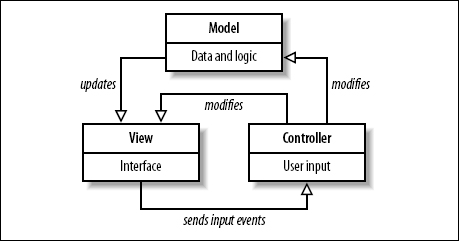
\includegraphics[width=0.7\textwidth, keepaspectratio]{img/designPattern/mvc.jpg}
		\caption{Esempio di applicazione del design pattern MVC}
	\end{center}
\end{figure}
\begin{itemize}
	\item \textbf{Scopo:} Disaccoppiare le tre seguenti componenti:
	\begin{itemize}
		\item Model: parte che si occupa direttamente di dati, logica e regole dell'applicazione;
		\item View: rappresentazione grafica sotto forma delle varie tipologie di output utilizzate per rappresentare i dati dell'applicazione;
		\item Controller: parte che accetta gli input e li converte in comandi per il model o la view;
	\end{itemize}
	 \item \textbf{Motivazione:} Molte applicazioni hanno la necessità di recuperare dati e di mostrarli in maniera opportuna agli utenti. Poiché si tratta di una comunicazione tra i dati dei dati e la interfaccia utente, bisogna trovare il metodo per far comunicare le due parti senza accorparle assieme, cosa che comporterebbe codice pesante e scarsa manutenibilità, in quanto in genere la parte grafica si evolve più in fretta della parte di model e, viceversa, bisogna rendere l'interfaccia che si offre all'utente quanto più separata possibile dall'implementazione effettiva della gestione dei dati. La soluzione che è stata trovata è costituita dal \gloss{design pattern} Model-View-Controller (MVC) che separa le tre componenti come già illustrato;
	 \item \textbf{Applicabilità:} Il pattern MVC è adatto ad essere utilizzato nei seguenti casi:
	 \begin{itemize}
	 	\item se c'è la necessità che un insieme di oggetti debba essere considerato come un oggetto singolo;
	 	\item se c'è la necessità di disaccoppiare il model e la view, creando un sistema di notifiche tra le due componenti;
	 	\item Se c'è la necessità di avere più view per il medesimo model.
\end{itemize}
\end{itemize}
\subsection{Design Pattern Creazionali}

\subsubsection{Singleton}

\begin{figure}[H]
  \begin{center}
    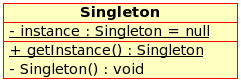
\includegraphics[width=0.3\textwidth, keepaspectratio]{img/designPattern/Singleton.png}
    \caption{Esempio di applicazione del design pattern singleton}
  \end{center}
\end{figure}

\begin{itemize}

\item \textbf{Scopo:} Assicurare che una classe abbia un'unica istanza ed avere
un punto di accesso globale ad essa;

\item \textbf{Motivazione:} Per alcune classi è fondamentale assicurare che non
abbiano più di un'istanza. Per questo motivo la classe tipicamente ha un
costruttore privato e un metodo per poter accedere all'istanza della classe
pubblico;

\item \textbf{Applicabilità:} Questo \gloss{design pattern} può essere
applicato nei seguenti casi:
   \begin{itemize}
   \item Quando è essenziale che ci sia solo una istanza di una classe e tale
   istanza deve essere resa accessibile attraverso un unico punto di accesso;
   \item Quando l'unica istanza della classe deve essere estesa in maniera
   tale da non dover avere \gloss{client} con codici diversi.
   \end{itemize}

\end{itemize}

\subsection{Design Pattern Strutturali}

\subsubsection{Façade}

\begin{figure}[H]
  \begin{center}
    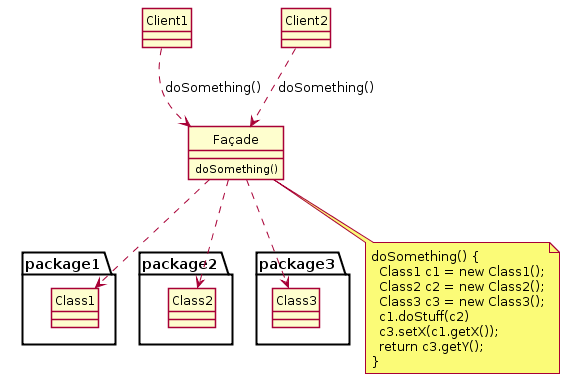
\includegraphics[width=0.7\textwidth, keepaspectratio]{img/designPattern/Facade.png}
    \caption{Esempio di applicazione del design pattern façade}
  \end{center}
\end{figure}

\begin{itemize}

\item \textbf{Scopo:} Semplificare l'interfaccia visibile all'utente di un sistema complesso.
Per fare ciò viene creata un'unica interfaccia che racchiude più classi, nascondendole all'esterno;

\item \textbf{Motivazione:} Raggruppare più sottosistemi in un sistema unico aiuta a ridurne la complessità.
L'utilizzo di una classe façade riduce le dipendenze tra i vari sottosistemi;

\item \textbf{Applicabilità:} Questo \gloss{design pattern} può essere
applicato nei seguenti casi:
  \begin{itemize}
  \item Quando c'è la necessità di avere una singola interfaccia semplice che raggruppi più sottosistemi;
  \item Quando c'è un alto livello di accoppiamento tra sottosistemi e client. La
  classe façade diminuisce queste dipendenze offrendo un'interfaccia singola;
  \item Quando si vogliono stratificare i sottosistemi con una struttura a livelli.
  \end{itemize}

\end{itemize}

\subsection{Design Pattern Comportamentali}

\subsubsection{Command}
\begin{figure}[H]
	\begin{center}
		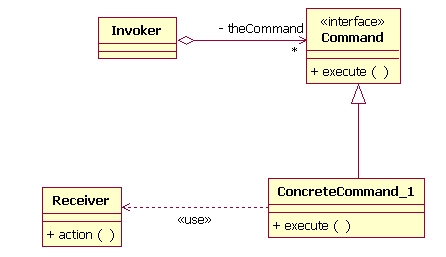
\includegraphics[width=0.7\textwidth, keepaspectratio]{img/designPattern/CommandPattern.png}
		\caption{Esempio di applicazione del design pattern command}
	\end{center}
\end{figure}
\begin{itemize}
	\item \textbf{Scopo:} Incapsulare una richiesta in un oggetto, cosicché il \gloss{client} sia indipendente dalle richieste, poiché le richieste hanno al loro interno tutti i dati necessari per essere risolte.
\item \textbf{Motivazione:} C'è la necessità di gestire richieste di cui non si conoscono i particolari poiché i Toolkit associano ai propri elementi, richieste da eseguire.
 Una classe astratta, Command, definisce l’interfaccia per eseguire la richiesta che è un semplice oggetto, per cui è possibile rendere variabile la reazione del \gloss{client} senza conoscere i dettagli dell'operazione stessa.
\item \textbf{Applicabilità:} Il Command pattern si presta bene alla parametrizzazione di oggetti sull’azione da eseguire (Callback function) soprattutto nello specificare, accodare ed eseguire richieste molteplici volte. Vi è inoltre il Supporto alle operazioni di "Undo" e "Redo". Vi è inoltre il supporto a transazione in quanto è possibile incapsulare un'azione in una operazione atomica.
\end{itemize}
\subsubsection{Iterator}
\begin{figure}[H]
	\begin{center}
		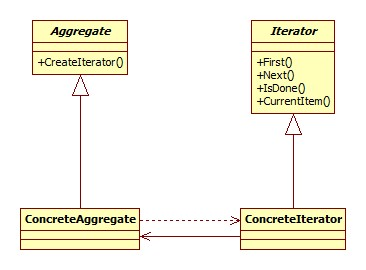
\includegraphics[width=0.7\textwidth, keepaspectratio]{img/designPattern/IteratorPattern.png}
		\caption{Esempio di applicazione del design pattern iterator}
	\end{center}
\end{figure}
\begin{itemize}
	\item \textbf{Scopo:} In un aggregato delegare la responsabilità dell'accesso da una classe separata dal contenitore stesso senza darne l'effettiva implementazione: si usa quindi l'iteratore, che fornisce metodi per navigare in maniera sequenziale attraverso il contenitore.
	\item \textbf{Motivazione:} Permette l'accesso ai dati nella medesima maniera dall'esterno e evita di appesantire il contenitore che altrimenti andrebbe arricchito di operazioni, rendendo il codice più complesso e difficilmente manutenibile. Inoltre permette di slegare il contenitore dalla maniera in cui si accede ad esso. Attraverso un iteratore si può inoltre ad esempio tenere traccia dell'elemento corrente, del precedente e del successivo.
	\item \textbf{Applicabilità:} Fornire l'accesso ad un aggregato senza fornire dettagli implementativi quali la struttura interna e la sua implementazione. Poiché rende  il contenitore indipendente dalla maniera in cui si percorre, esso è dunque aperto a diverse implementazioni per percorrerlo: è sufficente reimplementare l'iteratore, senza toccare il contenitore. Permette inoltre la presenza di più iteratori su uno stesso aggregato.
\end{itemize}
\subsubsection{Observer}
\begin{figure}[H]
	\begin{center}
		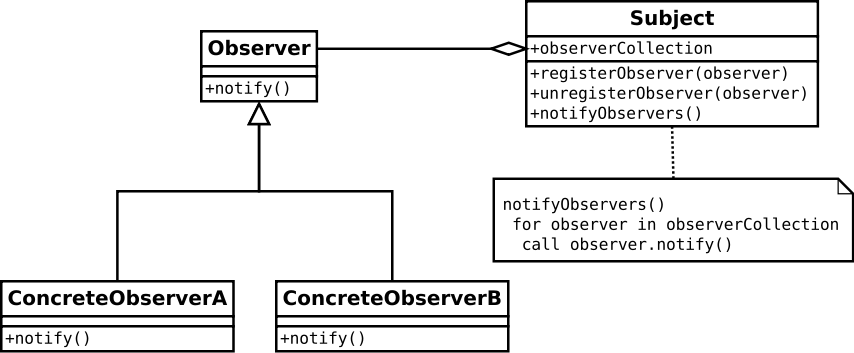
\includegraphics[width=0.7\textwidth, keepaspectratio]{img/designPattern/Observer.png}
		\caption{Esempio di applicazione del design pattern observer}
	\end{center}
\end{figure}
\begin{itemize}
\item \textbf{Scopo:} Definisce una dipendenza “1..n” fra oggetti, riflettendo la modifica di un oggetto su quelli che ad esso dipendono.
\item \textbf{Motivazione:} Mantenere la consistenza fra oggetti, oltre che al modello e alle viste ad esso collegate.
 Observer pattern definisce come implementare la relazione di dipendenza: infatti il modello prevede due  attori principali che sono:
 \begin{itemize}
 	\item Subject, che effettua le notifiche e contiene le interfacce per registrare e rimuovere gli observer;
 	\item Observer, che si aggiorna in base alle notifiche che riceve dal subject.
 \end{itemize}
\item \textbf{Applicabilità:} È utile nei casi in cui si debba associare più “viste” differenti ad una astrazione. Il pattern comporta inoltre un aumento del grado di riuso dei singoli tipi;
È indicato inoltre quando il cambiamento di un oggetto richiede il cambiamento di altri oggetti, oppure non si conosce quanti oggetti devono cambiare.
È utile anche per notificare oggetti senza fare assunzioni su quali siano questi oggetti ed evita l’accoppiamento “forte”.
\end{itemize}
\subsubsection{Strategy}
\begin{figure}[H]
	\begin{center}
		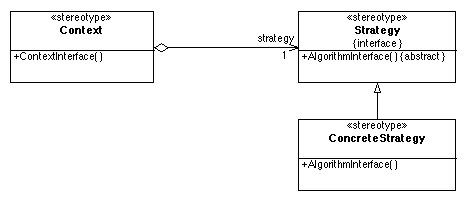
\includegraphics[width=0.7\textwidth, keepaspectratio]{img/designPattern/StrategyPattern.png}
		\caption{Esempio di applicazione del design pattern strategy}
	\end{center}
\end{figure}
\begin{itemize}
\item \textbf{Scopo:} Isolare un algoritmo all'interno di un oggetto, allo scopo di definire un gruppo di algoritmi, rendendoli
interscambiabili e indipendenti dal \gloss{client} che li utilizza. A questo proposito è necessario che la famiglia di algoritmi che implementa una stessa funzionalità esporti la medesima interfaccia in ogni caso, in questo modo il \gloss{client} che applica l'algoritmo non deve fare nessuna assunzioni sulla strategia applicata.
\item \textbf{Motivazione:} Esistono differenti algoritmi (strategie) che non possono essere inserite direttamente nel client. Infatti i \gloss{client}, senza l'utilizzo di questo pattern rischiano di divenire troppo complessi: differenti strategie sono appropriate in casi differenti e dover scrivere codice ogni volta è troppo gravoso. Inoltre, se non si utilizza questo \gloss{design pattern}, è difficile aggiungere nuovi algoritmi e modificare gli esistenti.
\item \textbf{Applicabilità:} questo \gloss{design pattern} si usa quando delle classi differiscono solo per il loro comportamento e si necessita di diverse varianti dello stesso algoritmo oppure quando una classe implementa diverse strategie attraverso molti statement condizionali, che si possono eliminare con questo \gloss{design pattern}. Inoltre l'iterator pattern si basa proprio su questo pattern.
\end{itemize}
\newpage
\listoftables
\newpage
\listoffigures
\end{document}
